\chapter{Convergence}

\marginpar{\red{Lecture 1}}

Probability theory is fundamentally concerned with asymptotic behavior as
the number of ``objects'' grows. Understanding probability therefore requires a
precise language for describing how sequences of random variables converge, and
for distinguishing the different senses in which such convergence may occur.

In this chapter we will introduce different notions of convergence and study how
they are related. The notion of convergence in \(L^p\) will lead us to the concept
of \(L^p\) spaces of random variables (Section \ref{sec: Lp spaces}). The
characterization of the strong notion of almost sure convergence, will lead us
to the Borel-Cantelli lemmas (Section \ref{sec: borel cantelli}).
In classical Analysis ``continuity'' is a central concept that allows
moving limits through functions and we will study whether this is also possible
in the probabilistic setting in Section \ref{sec: continuous mapping}.

Putting all these concepts together we will apply these concepts to
sums of random variables in the next chapter.

\section{Types of convergence}

In probability theory there are several different notions of convergence and in
this section we will define and relate them.

\begin{mdframed}[innertopmargin=0pt]
\begin{definition}[Types of Convergence]
    \label{def: types of convergence}
    A sequence of random variables \((X_n)_{n\in \nat}\) in a normed
    space \((\domain, \norm{\cdot})\) converges to a random variable \(X\)
    \begin{itemize}
        \item \textbf{almost surely}, or \textbf{with probability one}, denoted by \(X_n \overset{\as}\to X\), if
        \[
            \prob[\Big]{\lim_{n \to \infty} X_n = X} = 1.
        \]

        \item \textbf{in \(L^p\)} for \(p \geq 1\), denoted by \(X_n \overset{L^p}\to X\), if \(\E{\norm{X_n}^p} < \infty\) for all \(n\), \(\E{\norm{X}^p} < \infty\)
        and
        \[
            \lim_{n \to \infty} \E[\Big]{\norm{X_n - X}^p} = 0.
        \]

        \item \textbf{in probability}, denoted by \(X_n \overset{p}\to X\), if for all \(\epsilon > 0\)
        \[
            \lim_{n \to \infty} \prob[\big]{\norm{X_n- X} \ge \epsilon} = 0.
        \]

        \item \textbf{in distribution}, denoted by \(X_n \overset{d}\to X\), if
        it satisfies one of the following equivalent conditions (\textbf{Portemanteau theorem}):\nobreak
        \begin{enumerate}[label=(B.\arabic*),leftmargin=3em]
            \item\label{it: b.lip} For all \(f\colon \domain \to \real\) bounded, Lipschitz continuous we have \eqref{eq: fun convergence},
            \item\label{it: b.cont} For all \(f\colon \domain \to \real\) bounded, continuous we have \eqref{eq: fun
            convergence},
            \item\label{it: b.a.s. cont} For all \(f\colon \domain \to \real\) bounded, measurable, almost surely
            continuous in \(X\), that is \(\prob[\big]{f\text{
            continuous in }X} = 1\), we have \eqref{eq:
            fun convergence}.
        \end{enumerate}
        Where \eqref{eq: fun convergence} is given by
        \begin{equation}
            \label{eq: fun convergence}\tag{B}
            \lim_{n\to\infty}\E{f(X_n)} = \E{f(X)}.
        \end{equation}
        \begin{enumerate}[label=(S.\arabic*), nosep,leftmargin=3em]
            \item\label{it: s.closed} For all \underline{closed} sets \(A\) we have
            \[\limsup_{n\in \nat} \prob{X_n \in A} \le \prob{X \in A}.\]
            \item\label{it: s.open} For all \underline{open} sets \(O\) we have 
            \[\liminf_{n\in \nat }\prob{X_n \in O} \ge \prob{X \in O}.\]
            \item\label{it: s.zero boundary} For all \underline{measurable} sets \(B\) with \underline{\(\prob{X \in \partial B} = 0\)} we have
            \[
                \lim_{n \to \infty} \prob{X_n \in B} = \prob{X \in B}.
            \]
        \end{enumerate}
        If \(\domain = \real\) the following condition is also equivalent:
        \begin{enumerate}[label={(DF)},nosep,leftmargin=3em]
            \item\label{it: df} \textbf{Convergence of distribution functions}:
            for all \(x \in \real\) satisfying \(\prob{X = x} = 0\),
            \[
                \lim_{n \to \infty} \prob{X_n \leq x} = \prob{X \leq x}.
            \]
        \end{enumerate}
    \end{itemize}
    We say that two random variables \(X\) and \(Y\) are \textbf{almost surely equal},
    denoted by \(X \overset{\as}= Y\), if \(\prob{X = Y} = 1\).
    The limit \(X\) of a convergent sequence of random variables \((X_n)_{n\in \nat}\) is \textbf{almost
    surely unique}, if
    \[
        X_n \overset{(\cdot)}\to X \quad \text{and} \quad X_n \overset{(\cdot)}\to Y \implies X \overset{\as}= Y.
    \]
\end{definition}
\end{mdframed}

\begin{remark}[Generalization to metric spaces]
    Except for convergence in \(L^p\), the definitions may be extended in the
    obvious way to metric spaces \((\domain, \metric)\). We
    prove the Portemanteau theorem in this generalized setting.
\end{remark}

While the Portemanteau theorem may seem like it introduces many different
definitions, there are essentially just \textbf{two} equivalent concepts:
The first is \textbf{convergence of bounded functions in expectation} \eqref{eq: fun
convergence}, where the functions have different degrees of continuity. 
This is useful as it is sufficient to prove convergence for the smallest
class of Lipschitz functions to conclude convergence for the larger classes.
The second big concept is that the \textbf{probabilities of sets converge},
with the caveat that probability mass may converge outside the set at the boundary
of the set. As an example consider the deterministic sequence \(\prob{X_n =
\frac1n} =1\). Then we have \(\prob{X_n \in (0,1]} =1\) for all \(n\) but for
the limit \(X\) we have \(\prob{X = 0} = 1\).
Thus open sets may lose probability mass at the boundary, while closed sets
may gain probability mass at the boundary. If the boundary has zero mass
in the limit however, then the probabilities converge.
The convergence of distribution functions is just a special case, since
\[
    \prob{X_n \le x} = \prob{X_n \in (-\infty, x]}.
\]
So we simply consider the sets \((-\infty, x]\) for all \(x\in \real\)
for which the boundary \(\{x\}\) has zero probability mass in the limit.
The interesting thing about this special case is that it is enough to check
convergence on this small family of sets to conclude convergence of
a much larger family of sets.

With convergence in distribution reduced to these two big concepts
let us contextualize the other types of convergence before we get lost in the details of the proof
of the Portemanteau theorem. We summarize the implications
between the different types of convergence in the following theorem.
Notice the fundamental difference between convergence in distribution and the
other, stronger, types of convergence that have almost surely unique limits. To
see that convergence in distribution cannot have almost surely unique limits,
consider the fact that \(X\) and \(-X\) have the same distribution when the
distribution of \(X\) is symmetric (Exercise \ref{ex: unique stochastic limits}
\ref{it: non-unique limits convergence in dist}).

\begin{theorem}[Convergence implications]
    \label{thm: convergence implications}
    For a sequence of random variables \((X_n)_{n\in\nat}\) and a
    random variable \(X\) the following implications hold:
    \begin{center}
        \begin{tikzcd}[
    every matrix/.append style={name=m},
    cells={nodes={
        draw, 
        rectangle, 
        rounded corners, 
        align=center, 
        minimum width=2.5cm, 
        minimum height=0.8cm,
        inner sep=5pt
    }},
    % 2. Spacing between nodes
    row sep=0.7cm,
    column sep=1.7cm,
    % 3. Global Arrow Styling
    execute at end picture={
        \draw[dashed, thick, gray] 
        ($(m-1-2.north east)!0.5!(m-1-3.north west) + (0.1, 1.2)$) -- 
        ($(m-1-2.south east)!0.5!(m-1-3.south west) + (0.1, -2.3)$)
        node[midway, fill=white, text=gray, font=\footnotesize, xshift=-32,yshift=-53] {\(X\) a.s.\ unique};
    }
]
    % --- Row 1 ---
    |[yshift=20]| \(X_n \overset{\as}\to X\)
    % \parbox{2.1cm}{Almost sure convergence}
    \arrow[r, Rightarrow, out=0, in=170]{}{\text{\ref{it: as to p}}}
    \arrow[d,xshift=20]{}[left]{\substack{\text{MCT/DCT}\\\text{(Measure Theory)}}}
    & \(X_n \overset{p}\to X\)
    \arrow[r, Rightarrow] {}[xshift=-4]{\ref{it: p to d}}
    \arrow[l, out=180, in=352, looseness=1] {}[below,yshift=-5]{\substack{\text{Borel-Cantelli}\\Sec.~\ref{sec: borel cantelli}}}
    \arrow[ld, out=250, in=358] {} [right,xshift=4,yshift=-5]{\substack{\text{\(X_n,X\) bounded}\\\text{(Exercise \ref{ex: p to Lp when bounded})}}}
    & \(X_n \overset{d}\to X\)
    \arrow[l, out=220, in=345, looseness=1] {}[below,xshift=19]{X \overset{\as}= c \in \real \text{ \ref{it: d to p}}}
    \arrow[ll, out=140, in=50, looseness=0.3]{}[above]{\text{Skorokhod (Exercise \ref{ex: skorokhod representation})}}

    \\
    % --- Row 2 ---
    % The loop is defined here on the Lp node
    \(\;X_n \overset{L^p}\to X,\; p \ge 1\)
    \arrow[ur, Rightarrow, out=5, in=230] {}[above]{\text{\ref{it: L1 to p}}}
    \arrow[loop below, Rightarrow, looseness=3.5, out=220, in=290,xshift=-10]{}[xshift=15,yshift=-3]{L_q \overset{\ref{it: Lq to Lp}}\implies L_p \; (p \le q)}
    % & $L^1$ \text{ convergence} \arrow[u, Rightarrow] {} {\text{\ref{it: L1 to p}}}
\end{tikzcd}
    \end{center}
    \begin{enumerate}[label=(\arabic*),noitemsep]
        \item\label{it: as to p}
        If \(X_n \xrightarrow{\as} X\), then \(X_n \xrightarrow{p} X\).
        \item\label{it: p to d}
        If \(X_n \xrightarrow{p} X\), then \(X_n \xrightarrow{d} X\).
        \item \label{it: d to p}
        If \(X\) is deterministic, i.e.\ \(X \overset{\as}= c\in \real\), then
        \(X_n \xrightarrow{d} X\) implies \(X_n \xrightarrow{p} X\).
        \item\label{it: Lq to Lp}
        If \(X_n \xrightarrow{L^q} X\) for some \(q \ge p \ge 1\), then \(X_n \xrightarrow{L^p} X\).
        \item\label{it: L1 to p}
        If \(X_n \xrightarrow{L^1} X\), then \(X_n \xrightarrow{p} X\).
    \end{enumerate}
    See Exercises \ref{ex: convergence in distribution but not in probability},
    \ref{ex: convergence in probability but not in Lp}, \ref{ex: convergence in
    Lp but not as} and \ref{ex: as but not Lp} for counterexamples showing that
    we have not forgotten any true implications.
    \begin{enumerate}[label=(\arabic*),noitemsep, resume]
        \item\label{it: uniqueness of limits}
        The limits of convergence in probability are almost surely unique.
        Consequently, the same holds for stronger notions of convergence.
    \end{enumerate}
\end{theorem}

Observe that it is not possible to conclude convergence in probability 
from convergence in distribution if the limit is not almost surely constant.
Indeed, if the limit \(X\) is non-deterministic it can have different values.
It is therefore possible to construct two independent random variables \(X\) and \(Y\)
with the same distribution by essentially ``shuffling'' the outcomes and
letting \(X\) take a different value from \(Y\) since there are multiple
options. Since the limit is then not unique we cannot have convergence in
probability.

The remainder of this section is structured as follows: First, we will introduce
a few easy to prove tools. We will use them to prove the convergence implication
(Theorem \ref{thm: convergence implications}) but we will use these tools in other
sections as well. After proving these tools it is then natural to prove
Theorem \ref{thm: convergence implications} after which we will finally get
back to proving the Portemanteau theorem.

The first tool we introduce is the Markov inequality. It will become a very
close friend of ours as we will make frequent use of it (or its corollary)
in the following sections. It may be the most used inequality in probability
theory.

\begin{mdframed}[innertopmargin=0pt]
\begin{theorem}[Markov inequality]
    \label{thm: markov inequality}
    For an interval \(I\subseteq \real\) let \(h\colon I\to (0, \infty)\) be a
    non-decreasing function and \(X\) an \(I\)-valued random variable.
    Then for all \(t \in I\) we have
    \[
        \prob{X \ge t} \le \frac{\E{h(X)}}{h(t)}.
    \]
\end{theorem}
\begin{corollary}[Chebyshev inequality]
    \label{cor: markov inequality Lp}
    Let \(X\) be a random variable in a normed space \((\domain, \norm{\cdot})\)
    with \(\E{\norm{X}^p} < \infty\) for some \(p \ge 1\). Then
    \[
        \prob[\Big]{\norm{X - \E{X}} \ge t}
        \le \frac{\E[\Big]{\norm[\big]{X-\E{X}}^p}}{t^p}
        \qquad \text{for all }t > 0.
    \]
\end{corollary}
\end{mdframed}
\begin{remark}[Historical note]
    The case \(p=2\) is the classical ``Chebyshev inequality'', which
    is older than Markov's inequality.  Markov was Chebyshev's student and the
    classical ``Markov inequality'' is the one from Theorem \ref{thm: markov
    inequality} with \(h(x) = x\). The generalizations above are best known
    as Markov's inequality but also referred to as Chebyshev's inequality by
    some authors. We try to compromise with the Corollary covering a
    special case.
\end{remark}

\begin{proof}[Proof of Corollary \ref{cor: markov inequality Lp}]
    Markov inequality applied to \(\tilde X = \norm{X - \E{X}}\) 
    and \(h(x) = x^p\) with \(I = [0, \infty)\).
\end{proof}

\begin{proof}[Proof of Theorem \ref{thm: markov inequality}]
    Since \(h\) is non-decreasing and \(t, X \in I\)
    we have that \(X \ge t\) implies \(h(X) \ge h(t)\)
    and thus
    \[\begin{aligned}
        \prob{X \ge t}
        &\le \prob[\big]{h(X) \ge h(t)}
        = \E{\ind{h(X) \ge h(t)}}
        \le \E[\Big]{\frac{h(X)}{h(t)}\ind{h(X) \ge h(t)}}
        \\
        &\le \E[\Big]{\frac{h(X)}{h(t)}},
    \end{aligned}
    \]
    where we have used \(h > 0\) in the last inequality to remove the indicator.
\end{proof}

Before we get to the proof of Theorem \ref{thm: convergence implications}
we introduce another Lemma. A special case of the Lemma is the proof that
convergence in probability implies convergence in distribution but we will use
this more general form for the continuous mapping results (Section \ref{sec:
continuous mapping}).

\begin{lemma}\label{lem: moving target p to d}
    Let \((X_n)_{n\in \nat}\) and \((Y_n)_{n\in \nat}\) be two sequences of
    random variables in the metric space \((\domain, \metric)\) and
    \(f\colon \domain \to \real\) a bounded, Lipschitz continuous function, then
    \[
        \metric(X_n,Y_n) \overset{p}\to 0
        \quad\implies\quad
        \abs[\big]{\E{f(X_n)} - \E{f(Y_n)}} \to 0.
    \]
\end{lemma}

\begin{proof}
    Since \(f\) is bounded we have that \(\abs{f(x)} \le M\) for all \(x\in
    \domain\) for some \(M > 0\). Let \(L\) further be the Lipschitz constant
    of \(f\) and choose an arbitrary \(\epsilon > 0\).
    Then
    \[\begin{aligned}
        &\abs{\E{f(X_n)} - \E{f(Y_n)}}
        \\
        &\le \E{\abs{f(X_n) - f(Y_n)}}
        \\
        &\le \E{\underbrace{\abs{f(X_n) - f(Y_n)}}_{\le L\metric(X_n, Y_n)} \ind{\metric(X_n, Y_n) \le \epsilon}}
        + \E{\underbrace{\abs{f(X_n) - f(Y_n)}}_{\le 2M} \ind{\metric(X_n, Y_n) > \epsilon}}
        \\
        &\le L \epsilon + 2M \underbrace{\prob{\metric(X_n, Y_n) > \epsilon}}_{\to 0}.
    \end{aligned}\]
    Using \(\metric(X_n, Y_n) \overset{p}\to 0\) we thus we have \(\limsup_{n\to
    \infty} \abs{\E{f(X_n)} - \E{f(Y_n)}} \le L \epsilon\)
    for arbitrary \(\epsilon > 0\) and thus its limit must be zero.
\end{proof}

\begin{proof}[Proof (Theorem \ref{thm: convergence implications})]
    We will prove all implications not involving \(L^p\) for metric spaces. You
    may assume \(\metric(x,y) = \norm{x-y}\) for the sake of simplicity.
    \begin{enumerate}[wide=0pt]
        \item[\ref{it: p to d}] To see that Lemma \ref{lem: moving target p to d}
        proves that convergence in probability implies convergence in distribution,
        choose \(Y_n = X\) and observe that by definition
        \[
            \metric(X_n, X) \overset{p}\to 0 \iff X_n \overset{p}\to X
        \]
        then this Lemma proves \ref{it: b.lip} from the Portemanteau theorem.

        \item[\ref{it: L1 to p}] Convergence in probability may be easily deduced
        from the \(L^1\) Chebyshev inequality (Corollary
        \ref{cor: markov inequality Lp}): We have for \(\epsilon > 0\) \[
            \prob[\big]{\norm{X_n - X} > \epsilon}
            \le \frac{\E[\big]{\norm{X_n - X}}}{\epsilon}
            \to 0.
        \]

        \item[\ref{it: as to p}] To prove that almost sure convergence implies convergence in 
        probability observe that the set of point-wise convergence is given by
        \begin{align*}
            \set{X_n \to X}
            &= \set[\Big]{\omega \in \Omega : \lim_{n \to \infty} X_n(\omega) = X(\omega)}
            \\
            \overset{\text{def.}}&= \set[\Big]{
                \omega \in \Omega
                : \forall \epsilon > 0, \exists N\in \nat, \forall n \ge N
                : \metric(X_n(\omega), X(\omega)) < \epsilon}.
            \\
            &= \bigcap_{\epsilon > 0} \bigcup_{N \in \nat} \bigcap_{n \ge N}
            \set[\Big]{\omega \in \Omega : \metric(X_n(\omega), X(\omega)) < \epsilon}.
        \end{align*}
        By de Morgan's laws for set complements and almost sure
        convergence we therefore have
        \begin{align*}
            0 &= \prob[\big]{X_n \not\to X}
            \\
            &= \prob[\bigg]{\bigcup_{\epsilon > 0} \bigcap_{N \in \nat} \bigcup_{n \ge N}
            \set[\Big]{\omega \in \Omega : \metric(X_n(\omega), X(\omega)) \ge \epsilon}}
            \\
            \overset{\text{fix } \epsilon}&\ge \prob[\bigg]{\bigcap_{N \in \nat} \bigcup_{n \ge N}
            \set[\Big]{\omega \in \Omega : \metric(X_n(\omega), X(\omega)) \ge \epsilon}}
            \\
            &= \lim_{N \to \infty} \prob[\Big]{\bigcup_{n \ge N}
            \set[\Big]{\omega \in \Omega : \metric(X_n(\omega), X(\omega)) \ge \epsilon}}
            \\
            \overset{\text{fix } n=N}&\ge \lim_{N\to \infty} \prob[\big]{\metric(X_N, X) \ge \epsilon},
        \end{align*}
        where the penultimate equality follows from the continuity of the
        probability measure
        \[
            \lim_{N\to \infty} \prob{A_N} = \prob[\big]{\bigcap_{N\in \nat} A_N}
        \] for a decreasing sequence of
        events \(A_1 \supseteq A_2 \supseteq \ldots\)
        \continuityOfMeasure.

        \item[\ref{it: d to p}] Assume that \(X\equiv c\in \domain\), choose any
        \(\epsilon>0\) and let \(\ball{c}{\epsilon}\) denote the
        \(\epsilon\)-ball centered at \(c\).
        Then its border has zero probability under the distribution of \(X\), that is
        \(\prob{X\in \partial\ball{c}{\epsilon}} = 0\).
        Using \ref{it: s.zero boundary} from the Portemanteau theorem
        this implies
        \[
            \prob[\big]{\metric(X_n,X) < \epsilon}
            = \prob[\big]{X_n \in \ball{c}{\epsilon}}
            \to \prob[\big]{X \in \ball{c}{\epsilon}} = 1.
        \]
        Consequently \(\prob[\big]{\metric(X_n, X) \ge \epsilon} \to 0\).

        

        \item[\ref{it: Lq to Lp}] We will prove this implication in a separate
        section on \(L^p\) spaces (see Remark \ref{rem: Lp convergence} in
        Section \ref{sec: Lp spaces}).

        \item[\ref{it: uniqueness of limits}] See Exercise \ref{ex: unique stochastic limits}.
        \qedhere
    \end{enumerate}
\end{proof}

What remains is to prove the Portemanteau theorem as we have already made
use of different variants of convergence in distribution to prove the convergence
implications above.

\begin{myproof}[Proof (Portemanteau Theorem)]
    The proof strategy is as follows:
    \begin{center}
            \begin{tikzcd}[
        column sep=.6cm,
        row sep=0.5cm,
    ]
        \ref{it: b.a.s. cont}
        \arrow[r, Rightarrow]{}{\text{trivial}}
        & \ref{it: b.cont}
        \arrow[r, Rightarrow]{}{\text{trivial}}
        & \ref{it: b.lip}
        \arrow[r, Rightarrow]{}{!}
        & \ref{it: s.closed}
        \arrow[r, Leftrightarrow]{}{\text{easy}}
        & \ref{it: s.open}
        \arrow[r, Rightarrow]{}{\text{easy}}
        & \ref{it: s.zero boundary}
        \arrow[r, Rightarrow]{}{!}
        \arrow[d, Rightarrow]{}{\text{trivial}}
        & \ref{it: b.a.s. cont}.
        \\
        & & & & & \ref{it: df}
        \arrow[ul, Rightarrow]{}{!}
    \end{tikzcd}
    \end{center}
    The equivalence of \ref{it: s.open} and \ref{it: s.closed} follows from
    directly from set complements. These two conditions then imply \ref{it: s.zero boundary}
    by considering the interior and closure of the set \(B\) for an upper and lower
    bound.
    % Specifically, we have that \(\prob{X \in \closure{B}} = \prob{X \in B} = \prob{X\in \interior{B}}\)
    % as \(\prob{X \in \partial B} = 0\). This implies
    % \[\begin{aligned}
    %     \prob{X \in B} = \prob{X \in \interior{B}}
    %     &\le \liminf_{n\to \infty} \prob{X_n \in \interior{B}}
    %     \\
    %     &\le \lim_{n\to\infty} \prob{X_n \in B}
    %     \\
    %     &\le \limsup_{n\to \infty} \prob{X_n \in \closure{B}}
    %     \le \prob{X \in \closure{B}} = \prob{X \in B}.
    % \end{aligned}
    % \]

    % \begin{wrapstuff}[type=figure,width=.35\textwidth,top=1]
    %     \scalebox{0.7}{
    %     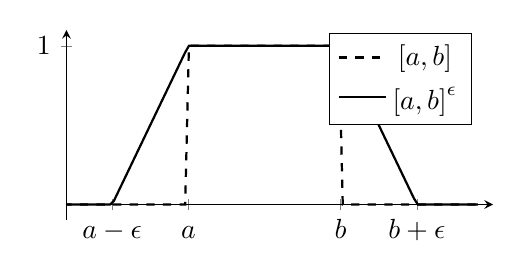
\begin{tikzpicture}
    \begin{axis}[
        axis lines=middle,
        xmin=0.2, xmax=3,
        ymin=-0.1, ymax=1.1,
        samples=200,
        domain=-2:2.9,
        width=7cm,
        height=4cm,
        legend style={at={(0.95,.5)}, anchor=south east},
        xtick={0.5, 1, 2, 2.5},
        ytick={0,1},
        xticklabels={\(a-\epsilon\), \(a\), \(b\), \(b+\epsilon\)},
        xticklabel style={text height=1.5ex}
    ]

    % Indicator function
    \addplot[
        thick,
        dashed
    ] {x <= 1 ? 0 : (x>2 ? 0: 1)};
    \addlegendentry{$\ind{[a,b]}$}

    % Lipschitz approximation
    \addplot[
        thick
    ] {
        x <= 0.5 ? 0 :
        (x >= 2.5 ? 0: 
        (x < 1 ? 2*(x-0.5) : 
        (x > 2 ? -2*(x-2) + 1 : 1)
        )
        )
    };
    \addlegendentry{$\ind{[a,b]}^{\vphantom{(}\epsilon}$}

    \end{axis}
\end{tikzpicture}
    %     }
    % \end{wrapstuff}

    \begin{wrapfigure}[5]{o}{0.35\textwidth}
        \scalebox{0.7}{
        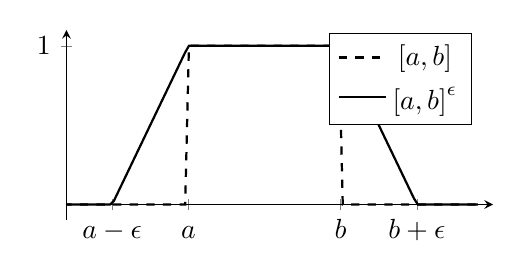
\begin{tikzpicture}
    \begin{axis}[
        axis lines=middle,
        xmin=0.2, xmax=3,
        ymin=-0.1, ymax=1.1,
        samples=200,
        domain=-2:2.9,
        width=7cm,
        height=4cm,
        legend style={at={(0.95,.5)}, anchor=south east},
        xtick={0.5, 1, 2, 2.5},
        ytick={0,1},
        xticklabels={\(a-\epsilon\), \(a\), \(b\), \(b+\epsilon\)},
        xticklabel style={text height=1.5ex}
    ]

    % Indicator function
    \addplot[
        thick,
        dashed
    ] {x <= 1 ? 0 : (x>2 ? 0: 1)};
    \addlegendentry{$\ind{[a,b]}$}

    % Lipschitz approximation
    \addplot[
        thick
    ] {
        x <= 0.5 ? 0 :
        (x >= 2.5 ? 0: 
        (x < 1 ? 2*(x-0.5) : 
        (x > 2 ? -2*(x-2) + 1 : 1)
        )
        )
    };
    \addlegendentry{$\ind{[a,b]}^{\vphantom{(}\epsilon}$}

    \end{axis}
\end{tikzpicture}
        }
        \caption{
            \(\epsilon\)-bump function example.
        }
    \end{wrapfigure}
    
    ``\ref{it: b.lip} \(\Rightarrow\) \ref{it: s.closed}'': We use \(\epsilon\)-bump
    functions as approximations of indicators.
    Specifically, using \(x_+ \coloneq \max\{x, 0\}\) we define
    \[
        \ind{A}^\epsilon(x) \coloneq \Bigl(1-\frac{\metric(x, A)}\epsilon\Bigr)_+,
    \]
    where the distance of \(x\) to the set \(A\) is
    defined as
    \[
        \metric(x,A) = \inf_{y\in A} \metric(x,y).
    \]
    Lipschitz continuity is straightforward to verify (Exercise \ref{ex: lipschitz bump functions}).
    Using an \(\epsilon\)-increase in size of the set \(A\)
    \[
        A_\epsilon \coloneq \set{x \in \domain : \metric(x,A) \le \epsilon}
        = A + \ball{0}{\epsilon},
    \]
    we have  \(\ind{A}(x) \le \ind{A}^\epsilon(x) \le \ind{A_\epsilon}(x)\) for all \(x\).
    Consequently we have for any closed set \(A\)
    \[\begin{aligned}
        \prob{X_n \in A} = \E{\ind{A}(X_n)}
        &\le \E{\ind{A}^\epsilon(X_n)}
        \\
        \overset{\ref{it: b.lip}}&\to \E{\ind{A}^\epsilon(X)} \le \E{\ind{A_\epsilon}(X)}
        = \prob{X \in A_\epsilon},
    \end{aligned}
    \]
    Thus for every \(\epsilon >0\) we have
    \(
        \limsup_{n\to \infty} \prob{X_n \in A} \le \prob{X \in A_\epsilon}.
    \)
    Since this is true for any \(\epsilon >0\) define
    \(B_m \coloneq A_{\frac1m}\), then we have
    \[
        \limsup_{n\to \infty} \prob{X_n \in A}
        \le \lim_{m\to\infty}\prob{X \in B_m}
        = \prob[\Big]{X \in \bigcap_{m\in \nat} B_m}
        = \prob{X \in A},
    \]
    where we recall that \(\lim_{N\to \infty}
    \prob{A_N} = \prob[\big]{\bigcap_{N\in \nat} A_N}\) for a decreasing
    sequence of events \(A_1 \supseteq A_2 \supseteq \ldots\)
    \continuityOfMeasure,
    and \(B_m \supseteq B_{m+1} \supseteq \dots\) with \(\bigcap_{m\in \nat} B_m = A\).

    ``\ref{it: s.zero boundary} \(\Rightarrow\) \ref{it: b.a.s. cont}'': For the
    opposite direction it is necessary to discretize a bounded, measurable,
    almost surely continuous function \(f\colon \domain \to \real\). For this discretization we want to
    select a finite number of \(y_0 \le \ldots \le y_N\) in \(\real\)
    such that 
    \begin{enumerate}[noitemsep]
        \item the bounded range of \(f\) is contained in the interval \([y_0, y_N)\),
        \item the \(y_i\) are an \(\epsilon\)-grid, i.e.\ \(y_{i+1} - y_i < \epsilon\) for all \(i\),
        \item \(\prob{f(X) = y_i} = 0\) for all \(i\).
    \end{enumerate}
    That the first two conditions can be satisfied is trivial by the boundedness of \(f\). For
    the third condition we observe that the set of points that do not
    satisfy this condition is at most countable
    \[
        \set[\big]{y \in \real : \prob{f(X) = y} > 0}
        = \bigcup_{k=1}^\infty \underbrace{\set[\Big]{y \in \real : \prob{f(X) = y} \ge \tfrac1k}}_{\text{at most \(k\)-many}}.
    \]
    Since there is thus an uncountable number of choices left we may assume that
    the \(y_i\) satisfy all three conditions.

    The third condition implies for \(E_i = [y_{i-1}, y_i)\) that
    \(\prob{f(X) \in \partial E_i} = 0\). We will now prove that this
    implies \(\prob{X \in \partial f^{-1}(E_i)} = 0\), which will
    allow us to apply \ref{it: s.zero boundary} to the sets \(f^{-1}(E_i)\).
    Let \(D_f\) be the set of discontinuities of \(f\). Then for any set \(A\)
    we claim to have
    \begin{equation}
        \label{eq: boundary inclusion}    
        \partial f^{-1}(A) \subseteq f^{-1}(\partial A) \cup D_f.
    \end{equation}
    \begin{center}
    \begin{tabular}{|p{0.9\textwidth}}
    To see this, let \(x \in \partial f^{-1}(A)\). If \(x\in D_f\) we are done
    so assume that \(f\) is continuous in \(x\). By definition of continuity
    there exists for any \(\epsilon > 0\) a \(\delta > 0\) such that
    \(f(\ball{x}{\delta}) \subseteq \ball{f(x)}{\epsilon}\). By definition of
    the boundary, there exists
    \[
        y \in f^{-1}(A) \cap \ball{x}{\delta}
        \quad \text{and}\quad
        z \in \bigl(f^{-1}(A)\bigr)^\complement \cap \ball{x}{\delta}.
    \]
    Since \(\bigl(f^{-1}(A)\bigr)^\complement = f^{-1}(A^\complement)\) we consequently
    have
    \[
        f(y) \in A \cap \ball{f(x)}{\epsilon}
        \quad \text{and}\quad
        f(z) \in A^\complement \cap \ball{f(x)}{\epsilon}.
    \]
    As neither set may thus be empty for any \(\epsilon > 0\), we have that
    \(f(x) \in \partial A\) and thus \(x \in f^{-1}(\partial A)\).
    \end{tabular}
    \end{center}
    With \eqref{eq: boundary inclusion} we conclude
    \[
        \prob{ X \in \partial f^{-1}(E_i)}
        \le \underbrace{\prob[\big]{X \in f^{-1}(\partial E_i)}}_{=\prob{f(X) \in \partial E_i}} + \underbrace{\prob{X \in D_f}}_{=0} = 0.
    \]
    Finally, we may use the discretization we built. Observe that if \(f(X_n)
    \in E_i\), then \(f(X_n) \le y_i\). Since the sets \(E_i\) cover
    the range of \(f\) we have
    \[
        \E{f(X_n)}
        \le \E[\Big]{\sum_{i=1}^N y_i \ind{E_i}(f(X_n))}
        = \sum_{i=1}^N y_i \underbrace{\prob{X_n \in f^{-1}(E_i)}}_{\overset{\ref{it: s.zero boundary}}\to \prob{X \in f^{-1}(E_i)}}
    \]
    where we use \(\prob{X \in \partial f^{-1}(E_i)} = 0\). Using \(y_i \le f(X) +
    \epsilon\) for \(f(X) \in E_i\) we get
    \[
        \sum_{i=1}^N y_i \prob{X \in f^{-1}(E_i)}
        = \E[\Big]{\sum_{i=1}^N y_i \ind{E_i}(f(X))}
        \le \E{f(X)} + \epsilon.
    \]
    Put together this implies
    \[
        \limsup_{n\to \infty} \E{f(X_n)}
        \le \E{f(X)} + \epsilon.
    \]
    As this is true for any \(\epsilon >0\) we may drop it. Applying the same
    arguments to \(-f\) we obtain the lower bound and consequently
    \(\E{f(X_n)} \to \E{f(X)}\).

    ``\ref{it: df} \(\Rightarrow\) \ref{it: b.lip}'':
    Let \(F(x) = \prob{X\le x}\) and \(F_n(x) = \prob{X_n \le x}\) be the
    distribution functions of \(X\) and \(X_n\). We need to deduce from
    \(F_n(x) \to F(x)\) for all \(x\in \real\) with \(\prob{X = x} = 0\) that
    \[
        \E{f(X_n)} \to \E{f(X)}
    \]
    for all bounded, Lipschitz continuous functions \(f\colon \real \to \real\).
    If \(f\) has Lipschitz constant \(L\), then by considering \(\frac1L f\) and
    linearity of the expectation we may assume without loss of generality that
    \(L=1\). Similarly, we may assume it is bounded by \(1\). Let \(\epsilon > 0\) and choose \(N\) large enough that it is possible to choose
    \(y_0 < \ldots < y_N\) such that
    \[
        F(y_0) \le \epsilon,\quad F(y_N) \ge 1 - \epsilon,
        \quad\text{and}\quad
        y_{i+1} - y_i < \epsilon\quad  \text{ for all } i.
    \]
    There are only countably many points where \(\prob{X = y} \neq 0\),
    since the number of points where \(\prob{X=y} \ge \tfrac1m\) is finite and a
    countable union (over \(m\)) of finite sets is countable.  We may therefore
    choose \(y_i\) such that \(\prob{X = y_i} = 0\) for all \(i\).
    For all \(x\in (y_{i-1}, y_i]\) we then have
    \[
        \abs{f(x) - f(y_i)} \overset{1\text{-Lip}}\le \abs{x-y_i} < \epsilon,
    \]
    and thus \(f(x) \le f(y_i) + \epsilon \le f(x)\). Recall that \(f\) is moreover bounded
    by \(1\) such that
    \[\begin{aligned}
        \E{f(X_n)}
        &\le \E{\ind{X_n \le y_0}} + \E[\Big]{\sum_{i=1}^N (f(y_i) +\epsilon)\ind{(y_{i-1}, y_i]}(X_n)}
        + \E{\ind{X_n > y_N}}
        \\
        &\le F_n(y_0) + \sum_{i=1}^N (f(y_i) + \epsilon) (F_n(y_i) - F_n(y_{i-1})) + (1 - F_n(y_N))
    \end{aligned}
    \]
    Since \(\lim_{n\to \infty} F_n(y_i) = F(y_i)\) for all \(i\) we consequently have
    \[\begin{aligned}
        \limsup_{n\to \infty} \E{f(X_n)}
        &\le \underbrace{F(y_0)}_{\le \epsilon} + \sum_{i=1}^N (f(y_i) + \epsilon) (F(y_i) - F(y_{i-1})) + \underbrace{(1 - F(y_N))}_{\le \epsilon}
        \\
        &\le 2\epsilon + \E[\Big]{\sum_{i=1}^N \underbrace{(f(y_i) + \epsilon)}_{\le f(X) + 2\epsilon} \ind{(y_{i-1}, y_i]}(X)}
        \\
        &\le 4\epsilon + \E{f(X)} - \E{f(X) \ind{X \le y_0}} - \E{f(X) \ind{X > y_N}}
        \\
        &\le 6\epsilon + \E{f(X)}.
    \end{aligned}
    \]
    Since \(\epsilon>0\) was arbitrary we thus obtain \(\limsup_{n\to \infty}
    \E{f(X_n)} \le \E{f(X)}\). Applying the same arguments to \(-f\) we get the
    lower bound.
\end{myproof}


\subsection*{Exercises \thesection}

% counterexample: convergence in distribution but not in probability

\begin{exercise}[Convergence in distribution but not probability \Coffeecup]
    \label{ex: convergence in distribution but not in probability}
    Let \(X\) be a random variable with \(\prob{X=-1} = \frac12\) and \(\prob{X=1}=\frac12\).
    \[
        X_n \coloneq (-1)^n X
    \]
    Prove that
    \begin{enumerate}[label=(\alph*), noitemsep]
        \item \(X_n \xrightarrow{d} X\)
        \begin{solution}
            Observe that the distribution of \(X\) is symmetric, that is
            \[
                \prob{-X \le x} = \prob{X \le x} \qquad \forall x\in \real.
            \]
            Consequently, for any \(x \in \real\) we have \(\prob{X_n \le x} = \prob{X \le x}\).
            In particular this implies \(\prob{X_n \le x} \to \prob{X \le x}\) for all \(x\).
        \end{solution}

        \item \(X_n\) does not converge in probability to \(X\).
        \begin{solution}
            We have for \(\epsilon = 1\) and every odd \(n\)
            \[
                \prob{\abs{X - X_n} \ge \epsilon}
                = \prob{2\abs{X} \ge 1} = 1
            \]
            The sequence \(\prob{|X_n - X| \ge \epsilon}\) thus does not converge to \(0\).
        \end{solution}
    \end{enumerate}
\end{exercise}



\begin{exercise}[Convergence in probability but not \(L^p\) \Coffeecup]
    \label{ex: convergence in probability but not in Lp}
    Let \(U\sim \uniform(0,1)\) be a standard uniform random variable and define
    \[
        X_n \coloneq n \ind{[0, 1/n)}(U)
    \]
    Show that
    \begin{enumerate}[label=(\alph*), noitemsep]
        \item the sequence \((X_n)_{n\in \nat}\) converges to \(0\) in probability,
        \begin{solution}
            We have for any \(\epsilon > 0\)
            \[
                \prob{|X_n - 0| \ge \epsilon}
                \le \prob(X_n \neq 0)
                = \prob[\big]{U\le \tfrac1n}
                = \tfrac1n
                \to 0.
                \qedhere
            \]
        \end{solution}

        \item the sequence \((X_n)_{n\in \nat}\) does not converge to \(0\) in \(L^1\),
        \begin{solution}
            We have
            \[
                \E{|X_n - 0|}
                = \E{X_n}
                = n \cdot \prob[\big]{U \in [0, 1/n)}
                = n \cdot \frac1n
                = 1 \not\to 0.
                \qedhere
            \]            
        \end{solution}

        \item For every \(p \ge 1\) construct a sequence \((Y_n)_{n\in \nat}\) such that
        \(Y_n\xrightarrow{L^q} 0\) for all \(q < p\) but not for \(q \ge p\).
        \begin{solution}
            Define \(Y_n \coloneq X_n^{1/p}\) with \(X_n\) as above. Then
            \[
                \E{|Y_n - 0|^q} = \E{X_n^{q/p}} = n^{q/p} \cdot \prob[\big]{U \in [0, 1/n)} = n^{q/p - 1}.
            \]
            This converges to \(0\) for all \(q < p\) but not for \(q \ge p\).
        \end{solution}
        \end{enumerate}
\end{exercise}


\begin{exercise}[Convergence in \(L^p\) but not almost surely \Coffeecup\Coffeecup] 
    \label{ex: convergence in Lp but not as}
    Let \(U\sim \uniform(0,1)\) be a standard uniform random variable.
    We will scan the interval for \(U\) with increasingly fine measurements. Specifically,
    let
    \begin{alignat*}{7}
        X_1 &\coloneq \ind{[0,1)}(U)
        \\
        X_2 &\coloneq \ind{[0,\frac12)}(U)
        \quad & X_3 &\coloneq \ind{[\frac12, 1)}(U)
        \\
        X_4 &\coloneq \ind{[0, \frac14)}(U)
        \quad & X_5 &\coloneq \ind{[\frac14, \frac12)}(U)
        \quad & X_6 &\coloneq \ind{[\frac12, \frac34)}(U)
        \quad & X_7 &\coloneq \ind{[\frac34, 1)}(U)
    \end{alignat*}
    That is
    \[
        X_n \coloneq \ind{\left[
            \frac{k}{2^{m}}, \frac{k+1}{2^{m}}
        \right)}(U),
        \quad \text{with}\quad 
        m \coloneq \lfloor\log_2(n)\rfloor, \quad k \coloneq n - 2^m. 
    \]
    Show that
    \begin{enumerate}[label=(\alph*), noitemsep]
        \item\label{it: (conv in Lp but not as) in Lp}
        \(X_n \xrightarrow{L^p} 0\),

        \item\label{it: (conv in Lp but not as) in prob}
        \(X_n \xrightarrow{p} 0\),

        \item\label{it: (conv in Lp but not as) not as}
        \(X_n\) does not converge almost surely to \(0\).
    \end{enumerate}
\end{exercise}
\begin{solution}
\begin{enumerate}[wide=0pt]
    \item[\ref{it: (conv in Lp but not as) in Lp}]
    We have for any \(p \ge 1\)
    \[
        \E{|X_n|^p} = \int_0^1 \ind{
            \left[\frac{k}{2^{m}}, \frac{k+1}{2^{m}} \right)
        }(u) \, du
        = \frac{1}{2^m} = 2^{-\lfloor \log_2(n) \rfloor} \to 0.
    \]
    Consequently, \(X_n \xrightarrow{L^p} 0\).

    \item[\ref{it: (conv in Lp but not as) in prob}]
    \(X_n \xrightarrow{L^p} 0\) implies \(X_n \xrightarrow{p} 0\) by Theorem
    \ref{thm: convergence implications} \ref{it: L1 to p}.

    Alternatively:
    \[
        \prob[\bigl]{|X_n - 0| \ge \epsilon}
        = \prob{X_n = 1}
        = 2^{-\lfloor \log_2(n) \rfloor} \to 0.
    \]
    for any \(\epsilon \in (0,1]\) and \(\prob[\bigl]{|X_n - 0| \ge
    \epsilon}=0\) for \(\epsilon > 1\).

    \item[\ref{it: (conv in Lp but not as) not as}]
    Choose any \(\omega \in \set{U\in [0,1)}\). We will show that there exists an
    \(\epsilon > 0\), specifically any \(\epsilon < 1\) such that
    \(|X_n(\omega) - 0| \ge \epsilon\) for infinitely many \(n\).
    Since we show this for any \(\omega\in \set{U\in [0,1)}\), this would imply
    \[
        \prob{X_n \not\to 0} \ge \prob{U \in [0,1)} = 1.
    \]
    For any \(N\in \nat\) the task is consequently to find \(n\ge N\)
    such that \(X_n(\omega) = 1\). Let \(m \coloneq \lfloor \log_2(N) \rfloor + 1\).
    Then there exists a \(k \in \{0, \ldots, 2^m-1\}\) such that
    \[
        \frac{k}{2^m} \le U(\omega) < \frac{k+1}{2^m}.
    \]
    Consequently, for \(n = 2^m + k\) we have \(n \ge N\) and
    \[
        X_n(\omega) = \ind{\left[
            \frac{k}{2^{m}}, \frac{k+1}{2^{m}}
        \right)}(U(\omega)) = 1.
        \qedhere
    \]
\end{enumerate}
\end{solution}


\begin{exercise}[subtitle={Stochastic convergence sometimes implies \(L^p\) \Coffeecup}]
    \label{ex: p to Lp when bounded}
    Assume that \(X_n\) and \(X\) are bounded random variables. That is 
    \(\sup_n\|X_n\| \le c\) and \(\|X\|\le c\) with probability one for some \(c
    \in \real\). Show that then \(X_n \overset{p}\to X\) implies \(X_n
    \overset{L^p}\to X\).
    \begin{remark}
        This is a weak form of the dominated convergence theorem, where the constant
        is the dominating function.
    \end{remark}
\end{exercise}
\begin{solution}
    We have for every \(\epsilon > 0\)
    \[\begin{aligned}
        \E[\big]{\norm{X_n - X}^p}
        &= \E[\big]{\norm{X_n - X}^p \ind{\norm{X_n - X} < \epsilon}}
        + \E[\big]{\norm{X_n - X}^p \ind{\norm{X_n - X} \ge \epsilon}}
        \\
        &\le \epsilon^p + (2c)^p \prob[\big]{\norm{X_n - X} \ge \epsilon}.
    \end{aligned}
    \]
    Due to \(X_n \overset{p}\to X\) the second term converges to \(0\)
    and we thus have
    \[
        \limsup_{n\to \infty} \E[\big]{\norm{X_n - X}^p} \le \epsilon^p.
    \]
    Since this is true for any \(\epsilon > 0\) we have the claim.
\end{solution}


\begin{exercise}[Stochastic triangle inequality \Coffeecup]
    \label{ex: stochastic triangle}
    Let \(X,Y,Z\) be random variables. Show for all \(\epsilon > 0\)
    \[
        \prob*{\norm{X - Z} \ge \epsilon} \le \prob*{\norm{X - Y} \ge \tfrac\epsilon2} + \prob*{\norm{Y - Z} \ge \tfrac\epsilon2}.
    \] 
    \textbf{Hint:} Use set inclusions.
    \begin{solution}
        The claim follows directly from
        \[
            \set{\norm{X - Z} \ge \epsilon}
            \subseteq \set{\norm{X - Y} \ge \tfrac\epsilon2} \cup \set{\norm{Y - Z} \ge \tfrac\epsilon2},
        \]
        which is proven using that \(A \subseteq B\) is equivalent
        to \(B^\complement \subseteq A^\complement\) and
        \begin{align*}
            \Bigl(\set{\norm{X - Y} \ge \tfrac\epsilon2} \cup \set{\norm{Y - Z} \ge \tfrac\epsilon2}\Bigr)^\complement
            &=\set{\norm{X - Y} < \tfrac\epsilon2} \cap \set{\norm{Y - Z} < \tfrac\epsilon2}
            \\
            &\subseteq \set{\norm{X - Z} < \epsilon}
            \\
            &= \set{\norm{X - Z} \ge \epsilon}^\complement.
        \end{align*}
        The standard triangle inequality is used for the inclusion step.
    \end{solution}
\end{exercise}


\begin{exercise}[Stochastic limits are unique \Coffeecup\Coffeecup]
    \label{ex: unique stochastic limits}
    Show that
    \begin{enumerate}[label=(\alph*),noitemsep]
        \item if \(X_n \overset{p}\to X\) and \(X_n \overset{p}\to Y\), then
        \(\prob{X = Y}=1\).

        \textbf{Hint:} How is uniqueness of limits proven in analysis?
        \begin{solution}
            We have for any \(\epsilon > 0\) and any \(n\in \nat\) by the
            stochastic triangle inequality (Exercise \ref{ex: stochastic
            triangle})
            \[\begin{aligned}
                \prob{\norm{X - Y} \ge \epsilon}
                \le \underbrace{\prob{\norm{X - X_n} \ge \tfrac\epsilon2}}_{\to 0} + \underbrace{\prob{\norm{X_n - Y} \ge \tfrac\epsilon2}}_{\to 0},
            \end{aligned}
            \]
            Since this inequality holds for any \(n\in \nat\) and \(X_n\)
            converges to both \(X\) and \(Y\) in probability, this term must
            therefore be equal to zero. That is \(\prob{\norm{X - Y} \ge
            \epsilon} = 0\) for any \(\epsilon > 0\). Since this is true for any
            \(\epsilon > 0\) we have by continuity of the probability measure
            \[
                \prob{X \neq Y} = \prob[\Big]{\bigcup_{n\in \nat}\norm{X - Y} > \frac1n} = \lim_{n\to\infty} \prob{\norm{X - Y} \ge \tfrac1n} = 0.
            \]
        \end{solution}
    \end{enumerate}
    Deduce
    \begin{enumerate}[label=(\alph*), resume,noitemsep]
        \item if \(X_n \overset{\as}\to X\) and \(X_n \overset{\as}\to Y\), then \(\prob{X = Y}=1,\)
        \item if \(X_n \overset{L^p}\to X\) and \(X_n \overset{L^p}\to Y\), then \(\prob{X = Y}=1.\)
        \begin{solution}
            If \(X_n \overset{\as}\to X\) and \(X_n \overset{\as}\to Y\), then
            \(X_n \overset{p}\to X\) and \(X_n \overset{p}\to Y\) by Theorem
            \ref{thm: convergence implications} \ref{it: as to p}. The claim
            then follows from the previous part. Similarly for \(L^p\) convergence.
        \end{solution}
    \end{enumerate}
    Finally, 
    \begin{enumerate}[label=(\alph*), resume, noitemsep]
        \item\label{it: non-unique limits convergence in dist} show that the statement is not true for convergence in
        distribution.

        \textbf{Hint:} Clearly \(X_n\) must converge in distribution but not
        in probability as the limits would otherwise be almost surely equal by the
        previous parts.

        \begin{solution}
            We may choose \(X\) as in Exercise \ref{ex: convergence in distribution but not in probability}.
            Since \(X_n \coloneq X\) converges both to \(X\) and \(-X\) in
            distribution the limit is clearly not unique as
            \[
                \prob{X = -X} = \prob{X=0}= 0.
                \qedhere
            \]
        \end{solution}
    \end{enumerate}
\end{exercise}

\begin{exercise}[subtitle={Stochastic Simulation and Quantiles \Coffeecup\Coffeecup}]
    \label{ex: stochastic simulation}
    The goal is to simulate a random variable \(X\) with distribution 
    function \(F(x) = \prob{X \le x}\) using a standard uniform random variable
    \(U\sim \uniform(0,1)\). We define the generalized inverse of \(F\) as
    \[
        F^{\leftarrow}(p) \coloneq \inf\{x \in \real : F(x) \ge p\}, \quad p \in (0,1).
    \]
    Show that
    \begin{enumerate}[label=(\alph*), noitemsep]
        \item\label{it: quantile if invertible}
        if \(F\) is invertible, then \(F^{\leftarrow}(p) = F^{-1}(p)\) for all
        \(p \in (0,1)\),

        \item\label{it: monotonicity}
        \(F^{\leftarrow}\) is non-decreasing,

        \item\label{it: F-(F(x)) le x}
        \(F^{\leftarrow}(F(x)) \le x\) for all \(x \in \real\),

        \item\label{it: F(F-(p)) > p}
        \(F(F^{\leftarrow}(p)) \ge p\) for all \(p \in (0,1)\),

        \item\label{it: F-(p)< x iff p<F(x)} \(F^{\leftarrow}(p) \le x\) if and only if \(p \le F(x)\),

        \item\label{it: inverse transform sampling}
        \(X\coloneq F^{\leftarrow}(U) \sim F\) for a standard uniform \(U\sim \uniform(0,1)\), i.e.\ 
        \[
            F(x) = \prob{X \le x}
            \qquad \forall x \in \real.
        \]

        \item\label{it: simulate exponential rvs} Propose a way to simulate an exponential distribution \(X \sim
        \exponential(\lambda)\) using a standard uniform random variable \(U\sim
        \uniform(0,1)\).
    \end{enumerate}
    The function \(F^{\leftarrow}\) is also called a \emph{quantile function} of
    the distribution function \(F\). The reason for this is
    the following: Show that
    \begin{enumerate}[resume, label=(\alph*), noitemsep]
        \item\label{it: quantiles}
         \(Q(p) \coloneq (-\infty, F^{\leftarrow}(p)]\) is the smallest
        interval of the form \((-\infty, a]\) such that \(\prob{X \in (-\infty,
        a]} \ge p\) for \(X\sim F\). We say that \(Q(p)\) is a \(p\)-quantile.
    \end{enumerate}
\end{exercise}
\begin{solution}
\begin{enumerate}[wide=0pt]
    \item[\ref{it: quantile if invertible}]
    Since \(F\) is monotonically increasing as a distribution
    function and additionally invertible, it is strict monotonically
    increasing. That is
    \[
        F(x) < F(y) \quad \text{for all } x < y.
    \]
    So clearly for all \(x< F^{-1}(p)\) we have \(F(x) < p\) and
    therefore they are not contained in the set \(\set{x\in \real : F(x)
    \ge p}\). This implies \(F^{-1}(p)\) is the smallest element in this set
    and consequently \(F^{\leftarrow}(p) = F^{-1}(p)\).

    \item[\ref{it: monotonicity}]
    Let \(p < q\). Then for any \(x \in \real\) such that \(F(x) \ge q\)
    we also have \(F(x) \ge p\). Consequently,
    \[
        \set{x \in \real : F(x) \ge q} \subseteq \set{x \in \real : F(x) \ge p},
    \]
    This implies the infimum of the former is greater than the infimum of the latter
    and thus
    \[
        F^{\leftarrow}(p) = \inf\{x \in \real : F(x) \ge p\} \le \inf\{x \in \real : F(x) \ge q\} = F^{\leftarrow}(q).
    \]

    \item[\ref{it: F-(F(x)) le x}]
    Since \(x\in \set{y\in \real : F(y) \ge F(x)}\), we have
    \[
        x \ge \inf\set{y\in \real : F(y) \ge F(x)} = F^{\leftarrow}(F(x)).
    \]

    \item[\ref{it: F(F-(p)) > p}]
    Let \(x_n \in \set{x\in \real : F(x) \ge p}\) be a sequence with \(x_n \downarrow F^{\leftarrow}(p)\). Then
    by right-continuity of the distribution function \(F\)
    \[
        p \le \lim_{n\to \infty} F(x_n)
        = F\Bigl(\lim_{n\to \infty} x_n\Bigr)
        = F(F^{\leftarrow}(p)).
    \]
    
    \item[\ref{it: F-(p)< x iff p<F(x)}]
    Assume \(F^{\leftarrow}(p) \le x\). Then by \ref{it: F(F-(p)) > p} 
    and the monotonicity of \(F\) we have
    \[
        p \overset{\ref{it: F(F-(p)) > p}}\le F(F^{\leftarrow}(p)) \le F(x).
    \]
    For the opposite direction assume \(p\le F(x)\), then by the
    monotonicity of \(F^{\leftarrow}\) \ref{it: monotonicity}
    and \ref{it: F-(F(x)) le x} we have
    \[
        F^{\leftarrow}(p) \overset{\ref{it: monotonicity}}\le F^{\leftarrow}(F(x)) \overset{\ref{it: F-(F(x)) le x}}\le x.
    \]

    \item[\ref{it: inverse transform sampling}]
    We simply use \ref{it: F-(p)< x iff p<F(x)} and the definition of \(U\) to get
    \[
        \prob{X \le x}
        = \prob{F^{\leftarrow}(U) \le x}
        \overset{\ref{it: F-(p)< x iff p<F(x)}}\le \prob{U \le F(x)}
        = \int_0^{F(x)} 1 \, du
        = F(x).
    \]

    \item[\ref{it: simulate exponential rvs}]
    The CDF of an exponential distribution is \(F(x) = 1 - e^{-\lambda x}\) for \(x \ge 0\).
    Since this function is invertible on \([0, \infty]\) we use
    \ref{it: quantile if invertible}. To get
    \[
        F^{\leftarrow}(p) = -\tfrac{1}{\lambda} \log(1-p).
    \]
    Using \(U \sim \uniform(0,1)\) we thus set \(X = F^{\leftarrow}(U)\),
    and finish by \ref{it: inverse transform sampling}.

    \item[\ref{it: quantiles}]
    For any \(a < F^{\leftarrow}(p)\) we have by definition of \(F^{\leftarrow}\) that
    \(F(a) < p\) and thus
    \[
        \prob{X \in (-\infty, a]} = F(a) < p.
    \]
    However for \(a=F^{\leftarrow}(p)\) we have \(F(a)\ge p\) by
    \ref{it: F(F-(p)) > p}.  Consequently, \(F^{\leftarrow}(p)\) is the
    smallest \(a\) such that \(\prob{X \in (-\infty, a]} \ge p\).
    \qedhere
\end{enumerate}
\end{solution}

\begin{exercise}[subtitle={Monotone functions have countable discontinuities \Coffeecup\Coffeecup\Coffeecup}]
    \label{ex: monotone functions have countably many discontinuities}
    Let \(F\colon \real \to \real\) be a non-decreasing function.
    \begin{enumerate}[label=(\alph*), noitemsep]
        \item\label{it: (monotone functions) left and right limits}
        Let \(x\in \real\). Prove that the limit
        \[
            F_-(x) \coloneq \lim_{n\to \infty} F(x_n)
        \]
        exists for any sequence \((x_n)_{n\in \nat} \subseteq \real\) with \(x_n < x\)
        and \(x_n \to x\). Prove that this limit is the same for any such
        sequence such that \(F_-(x)\) is well-defined.
        Also prove that \(F_+(x) \coloneq \lim_{y\downarrow x} F(y)\) is
        well-defined.

        \textbf{Hint:} Consider monotonically increasing sequences \(x_n\) first.
        Then prove that the liminf and limsup coincide for general sequences
        using monotone subsequences.

        \item\label{it: F continuous if and only if all coincide}
        Prove that \(F\) is continuous at \(x\) if and only
        if \(F(x) = F_-(x) = F_+(x)\). That is
        \(F\) only has jump discontinuities.

        \item\label{it: (monotone functions) countable jumps, compact interval}
        Prove that \(F\) restricted to a compact interval \([a,b]\)
        has only countably many jumps (places where \(F_-(x) < F_+(x)\)).

        \textbf{Hint:} How many jumps are there of size greater than \(1/n\)?

        \item\label{it: (monotone functions) countable jumps, real line}
        Prove that \(F\) has at most countably many discontinuities.
    \end{enumerate}
\end{exercise}

\begin{solution}
\begin{enumerate}[wide=0pt]
    \item[\ref{it: (monotone functions) left and right limits}]
    Let \(x_n\uparrow x\) be a monotonically increasing sequence. Then
    \(F(x_n)\) is also monotonically increasing and thus assumes a limit.
    We will prove \(\lim_n F(x_n) \le \lim_n F(y_n)\)
    for another monotonically increasing sequence \(y_n\uparrow x\).
    Since \(x_n\) and \(y_n\) are exchangeable we then also have equality.
    Now for any \(n\in \nat\) there exists an \(m_n\in \nat\) such that
    \(x_n \le y_{m_n} \le x\) as \(x_n < x\) and \(y_n\to x\). Consequently
    since \(F\) is non-decreasing we have
    \[
        \lim_{n\to\infty} F(x_n) \le \lim_{n\to\infty}F(y_{m_n}) \overset{\text{subsequence}}= \lim_{n\to\infty}F(y_n).
    \]
    Thus we have proven that the limit of monotonically increasing
    sequences is unique and denoted by \(F_-(x)\). Let \(x_n \to x\) with \(x_n < x\) be an
    arbitrary sequence. Let \(x_{n_k}\) be a subsequence with
    \[
        F(x_{n_k}) \to \liminf_{n\to\infty} F(x_n)
    \]
    Since \(x_{n_k} \to x\) and \(x_{n_k} < x\) we can find a monotonically increasing subsequence.
    This subsequence converges to \(F_-(x)\) and since it must have the
    same limit as the original sequence \(x_{n_k}\) we have
    \[
        \liminf_{n\to\infty} F(x_n) = F_-(x).       
    \]
    The same argument works for the limsup. Thus the limit exists and is
    given by \(F_-(x)\). The exact same argument also works for
    \(F_+(x)\) with decreasing sequences.

    \item[\ref{it: F continuous if and only if all coincide}]
    Clearly we have \(F_-(x) = F_+(x)\) if \(F\) is continuous.  So we
    only need to prove \(F\) continuous in \(x\) when this equality
    holds true.  Note that
    \(F_-(x) \le F(x) \le F_+(x)\) since \(F\) is non-decreasing.
    So if we have the equality then by a sandwich argument they are
    both equal to \(F(x)\). Let us assume equality. To prove
    sequential continuity in \(x\) we choose a sequence \(x_n\to x\).
    This sequence can be split into the parts that are smaller than \(x\)
    converging to \(F_-(x)\), the parts that are equal to \(x\),
    converging to \(F(x)\) and the parts that are larger than \(x\)
    converging to \(F_+(x)\). Since all these limits coincide the entire
    sequence converges to \(F(x)\). Consequently \(F\) is continuous in
    \(x\).

    \item[\ref{it: (monotone functions) countable jumps, compact interval}]
    Since \(F(b) - F(a)\) is finite and \(F\) monotonically increasing,
    there are at most \(\lceil n(F(b)-F(a))\rceil\) jumps of size
    \(\frac1n\). Thus for any \(n\in \nat\) the number of jumps of greater
    size is finite. This implies that the discontinuity set
    \[
        D_F = \set{x: F_-(x) \neq F_+(x)} = \bigcup_{n\in \nat} \set[\big]{x: F_+(x) - F_-(x) > \tfrac1n}
    \]
    is countable.

    \item[\ref{it: (monotone functions) countable jumps, real line}]
    Since \(F\) only has countably many discontinuities in each
    interval \([n, n+1]\) for \(n\in \integer\) and the countable union
    of countable sets is countable, we have that the set of all
    discontinuities is at most countable.
\end{enumerate}
\end{solution}


\begin{exercise}[Discontinuity points of distribution functions \Coffeecup\Coffeecup]
    Let \(X\) be a random variable and \(F(x) = \prob{X \le x}\) its
    distribution function. Show that \(F\) is continuous at \(x\) if and only if
    \(\prob{X = x} = 0\).
    \textbf{Hint:} Use Exercise \ref{ex: monotone functions have countably many discontinuities}.
\end{exercise}
\begin{solution}
    Since the sets \(\set{X \le x - \frac1n}\) are increasing
    in size, we have by continuity of the probability measure
    \[
        \prob{X < x}
        = \prob[\Big]{\bigcup_{n\in \nat} \set{X \le x - \tfrac1n}}
        = \lim_{n\to\infty} \prob{X \le x - \tfrac1n}
        = F_-(x).
    \]
    Consequently,
    \[
        \prob{X = x} = \prob{X \le x} - \prob{X < x} = F(x) - F_-(x).
    \]
    By Exercise \ref{ex: monotone functions have countably many
    discontinuities} \ref{it: F continuous if and only if all coincide} we
    have that \(F\) is continuous at \(x\) if and only if \(F(x) = F_-(x)\).
    Consequently continuity of \(F\) is equivalent to \(\prob{X = x} = 0\).
\end{solution}

\begin{exercise}[Skorokhod's representation theorem \Coffeecup\Coffeecup]
    \label{ex: skorokhod representation}
    Let \((X_n)_{n \in \nat}\) be a sequence of random variables in \(\real\)
    such that \(X_n \xrightarrow{d} X\). Show that there exist random variables
    \((Y_n)_{n\in \nat}\) and \(Y\), where the \(Y_n\) and \(Y\) are all defined on the
    same probability space such that
    \begin{enumerate}[label=(\roman*), noitemsep]
        \item \(Y_n \overset{d}= X_n\) for all \(n\in \nat\) and \(Y \overset{d}= X\),
        \item \(Y_n \overset{\as}\to Y\).
    \end{enumerate}
    \textbf{Hint:} Use \(F_n(x) = \prob{X_n \le x}\), Exercise \ref{ex:
    stochastic simulation} and that a monotonous function has at most countably
    many discontinuities (Exercise \ref{ex: monotone functions have countably
    many discontinuities}).
    \begin{remark}
        We assume \(X_n\) in \(\real\) to simplify the proof. Skorokhod's representation 
        theorem holds in much greater generality.
    \end{remark}
\end{exercise}
\begin{solution}
    Choose \(U\sim \uniform(0,1)\) and define
    \[
        Y_n \coloneq F_n^{\leftarrow}(U)
        \quad \text{and}\quad
        Y = F^{\leftarrow}(U)
    \] where \(F_n\) are the distribution functions of \(X_n\) and \(F\) the
    one of \(X\). Then by Exercise \ref{ex: stochastic simulation} we have
    \(Y_n \overset{d}= X_n\) for all \(n\in \nat\) and
    \(Y \overset{d}= X\).  It remains to show that \(Y_n \overset{\as}\to
    Y\). Since \(X_n \overset{d}\to X\) in distribution, we have that
    \(F_n(x) \to F(x)\) for all \(x\in \real\) at which \(F\) is continuous.
    Since the set \(D_F\) of discontinuity points of \(F\) is countable, we have
    \[
        \prob{U \in D_F} = \sum_{x\in D_F}\prob{U = x} = 0.
    \]
    And for all \(\omega \in \set{U \notin D_F}\) we have
    \[
        Y_n(\omega) = F_n(U(\omega)) \to F(U(\omega))=Y(\omega)
    \]
    Consequently, \(\prob{ Y_n \to Y } = \prob{U \notin D_F} = 1\) and thus \(Y_n \overset{\as}\to Y\).
\end{solution}


\begin{exercise}[Lipschitz continuous bump functions \Coffeecup\Coffeecup]
    \label{ex: lipschitz bump functions}
    Let \((\domain, \metric)\) be a metric space and \(A \subseteq \domain\). 
    Show that
    \begin{enumerate}[label=(\alph*)]
        \item \(x\mapsto \metric(x,A)\coloneq \inf_{z \in A} \metric(x,z)\) is \(1\)-Lipschitz continuous.
        \begin{solution}
        By the triangle inequality we have for \(x,y\in \domain\)
        \[
            \metric(x,A)
            =\inf_{z\in A} \metric(x,z)
            \le \inf_{z\in A} \bigl(\metric(x,y) + \metric(y,z)\bigr)
            = \metric(x,y) + \metric(y,A).
        \]
        with reordering this implies
        \[
            \metric(x,A) - \metric(y,A) \le \metric(x,y)
        \]
        By symmetry we also have  \(\metric(y,A) - \metric(x,A) \le \metric(x,y)\)
        and thereby the claim.
        \end{solution}

        \item \(x\mapsto x_+ = \max\set{x,0}\) is \(1\)-Lipschitz continuous.
        \begin{solution}
            Choose \(x,y\in \real\), without loss of generality
            assume \(x \ge y\). If \(y\le x\le 0\), then \(x_+ = y_+ = 0\) and thus
            \(
                \abs{x_+ - y_+} = 0 \le \abs{x-y}. 
            \)

            If \(x\ge 0\), then
            \(
                \abs{x_+ - y_+} = x - y_+ \le x-y = \abs{x-y}.
            \)
        \end{solution}

        \item If \(f\) is \(L_1\)-Lipschitz continuous and \(g\) is \(L_2\)-Lipschitz continuous, then
        \(f\circ g\) is \(L_1L_2\)-Lipschitz continuous.
        \begin{solution}
            We have for any \(x,y\in \domain\)
            \[
                \abs{f(g(x)) - f(g(y))}
                \le L_1 \abs{g(x) - g(y)}
                \le L_1L_2 \abs{x-y}.
                \qedhere
            \]
        \end{solution}


        \item the bump function \(\ind{A}^\epsilon(x) = (1 - \frac{\metric(x,A)}\epsilon)_+\)
        is \(\frac1\epsilon\)-Lipschitz continuous.
        \begin{solution}
            \(f_1(x) = \metric(x,A)\) is \(1\)-Lipschitz continuous,
            \(f_2(x) = 1 - \frac{x}{\epsilon}\) is \(\frac1\epsilon\)-Lipschitz continuous
            as a Linear function, and \(f_3(x) = x_+\) is \(1\)-Lipschitz continuous. Consequently
            \[
                f_3 \circ f_2 \circ f_1(x) = \ind{A}^\epsilon(x)
            \]
            is \(\frac1\epsilon\)-Lipschitz continuous by the previous part.
        \end{solution}
    \end{enumerate}
\end{exercise}


\begin{exercise}[How to check ``Equal in distribution'' \Coffeecup]
    \label{ex: equal in distribution}
    Let \(X\) and \(Y\) be two random variables in a metric space \(\domain\) with
    \begin{equation}
        \label{eq: equal in distribution}    
        \E{f(X)} = \E{f(Y)}
    \end{equation}
    for all bounded (measurable) functions \(f\colon \domain \to \real\). Show
    that this implies that \(X\) and \(Y\) are equal in distribution, that is
    \[
        \prob{X \in A} = \prob{Y \in A}
    \]
    for all (measurable) sets \(A\subseteq \domain\).
    
\begin{remark}
    Observe that this is very similar to Portemanteu's theorem (cf.~Definition
    \ref{def: types of convergence}) that characterizes convergence in
    distribution. And it can be shown that it is enough to check \eqref{eq:
    equal in distribution} for all bounded and Lipschitz functions \(f\colon
    \domain \to \real\).
\end{remark}
    \begin{solution}
        \(\ind{A}\) is a bounded and measurable function for any measurable set \(A\subseteq \domain\).
    \end{solution}
\end{exercise}



\subsection*{Exercises \thesection}

% counterexample: convergence in distribution but not in probability

\begin{exercise}[Convergence in distribution but not probability \Coffeecup]
    \label{ex: convergence in distribution but not in probability}
    Let \(X\) be a random variable with \(\prob{X=-1} = \frac12\) and \(\prob{X=1}=\frac12\).
    \[
        X_n \coloneq (-1)^n X
    \]
    Prove that
    \begin{enumerate}[label=(\alph*), noitemsep]
        \item \(X_n \xrightarrow{d} X\)
        \begin{solution}
            Observe that the distribution of \(X\) is symmetric, that is
            \[
                \prob{-X \le x} = \prob{X \le x} \qquad \forall x\in \real.
            \]
            Consequently, for any \(x \in \real\) we have \(\prob{X_n \le x} = \prob{X \le x}\).
            In particular this implies \(\prob{X_n \le x} \to \prob{X \le x}\) for all \(x\).
        \end{solution}

        \item \(X_n\) does not converge in probability to \(X\).
        \begin{solution}
            We have for \(\epsilon = 1\) and every odd \(n\)
            \[
                \prob{\abs{X - X_n} \ge \epsilon}
                = \prob{2\abs{X} \ge 1} = 1
            \]
            The sequence \(\prob{|X_n - X| \ge \epsilon}\) thus does not converge to \(0\).
        \end{solution}
    \end{enumerate}
\end{exercise}



\begin{exercise}[Convergence in probability but not \(L^p\) \Coffeecup]
    \label{ex: convergence in probability but not in Lp}
    Let \(U\sim \uniform(0,1)\) be a standard uniform random variable and define
    \[
        X_n \coloneq n \ind{[0, 1/n)}(U)
    \]
    Show that
    \begin{enumerate}[label=(\alph*), noitemsep]
        \item the sequence \((X_n)_{n\in \nat}\) converges to \(0\) in probability,
        \begin{solution}
            We have for any \(\epsilon > 0\)
            \[
                \prob{|X_n - 0| \ge \epsilon}
                \le \prob(X_n \neq 0)
                = \prob[\big]{U\le \tfrac1n}
                = \tfrac1n
                \to 0.
                \qedhere
            \]
        \end{solution}

        \item the sequence \((X_n)_{n\in \nat}\) does not converge to \(0\) in \(L^1\),
        \begin{solution}
            We have
            \[
                \E{|X_n - 0|}
                = \E{X_n}
                = n \cdot \prob[\big]{U \in [0, 1/n)}
                = n \cdot \frac1n
                = 1 \not\to 0.
                \qedhere
            \]            
        \end{solution}

        \item For every \(p \ge 1\) construct a sequence \((Y_n)_{n\in \nat}\) such that
        \(Y_n\xrightarrow{L^q} 0\) for all \(q < p\) but not for \(q \ge p\).
        \begin{solution}
            Define \(Y_n \coloneq X_n^{1/p}\) with \(X_n\) as above. Then
            \[
                \E{|Y_n - 0|^q} = \E{X_n^{q/p}} = n^{q/p} \cdot \prob[\big]{U \in [0, 1/n)} = n^{q/p - 1}.
            \]
            This converges to \(0\) for all \(q < p\) but not for \(q \ge p\).
        \end{solution}
        \end{enumerate}
\end{exercise}


\begin{exercise}[Convergence in \(L^p\) but not almost surely \Coffeecup\Coffeecup] 
    \label{ex: convergence in Lp but not as}
    Let \(U\sim \uniform(0,1)\) be a standard uniform random variable.
    We will scan the interval for \(U\) with increasingly fine measurements. Specifically,
    let
    \begin{alignat*}{7}
        X_1 &\coloneq \ind{[0,1)}(U)
        \\
        X_2 &\coloneq \ind{[0,\frac12)}(U)
        \quad & X_3 &\coloneq \ind{[\frac12, 1)}(U)
        \\
        X_4 &\coloneq \ind{[0, \frac14)}(U)
        \quad & X_5 &\coloneq \ind{[\frac14, \frac12)}(U)
        \quad & X_6 &\coloneq \ind{[\frac12, \frac34)}(U)
        \quad & X_7 &\coloneq \ind{[\frac34, 1)}(U)
    \end{alignat*}
    That is
    \[
        X_n \coloneq \ind{\left[
            \frac{k}{2^{m}}, \frac{k+1}{2^{m}}
        \right)}(U),
        \quad \text{with}\quad 
        m \coloneq \lfloor\log_2(n)\rfloor, \quad k \coloneq n - 2^m. 
    \]
    Show that
    \begin{enumerate}[label=(\alph*), noitemsep]
        \item\label{it: (conv in Lp but not as) in Lp}
        \(X_n \xrightarrow{L^p} 0\),

        \item\label{it: (conv in Lp but not as) in prob}
        \(X_n \xrightarrow{p} 0\),

        \item\label{it: (conv in Lp but not as) not as}
        \(X_n\) does not converge almost surely to \(0\).
    \end{enumerate}
\end{exercise}
\begin{solution}
\begin{enumerate}[wide=0pt]
    \item[\ref{it: (conv in Lp but not as) in Lp}]
    We have for any \(p \ge 1\)
    \[
        \E{|X_n|^p} = \int_0^1 \ind{
            \left[\frac{k}{2^{m}}, \frac{k+1}{2^{m}} \right)
        }(u) \, du
        = \frac{1}{2^m} = 2^{-\lfloor \log_2(n) \rfloor} \to 0.
    \]
    Consequently, \(X_n \xrightarrow{L^p} 0\).

    \item[\ref{it: (conv in Lp but not as) in prob}]
    \(X_n \xrightarrow{L^p} 0\) implies \(X_n \xrightarrow{p} 0\) by Theorem
    \ref{thm: convergence implications} \ref{it: L1 to p}.

    Alternatively:
    \[
        \prob[\bigl]{|X_n - 0| \ge \epsilon}
        = \prob{X_n = 1}
        = 2^{-\lfloor \log_2(n) \rfloor} \to 0.
    \]
    for any \(\epsilon \in (0,1]\) and \(\prob[\bigl]{|X_n - 0| \ge
    \epsilon}=0\) for \(\epsilon > 1\).

    \item[\ref{it: (conv in Lp but not as) not as}]
    Choose any \(\omega \in \set{U\in [0,1)}\). We will show that there exists an
    \(\epsilon > 0\), specifically any \(\epsilon < 1\) such that
    \(|X_n(\omega) - 0| \ge \epsilon\) for infinitely many \(n\).
    Since we show this for any \(\omega\in \set{U\in [0,1)}\), this would imply
    \[
        \prob{X_n \not\to 0} \ge \prob{U \in [0,1)} = 1.
    \]
    For any \(N\in \nat\) the task is consequently to find \(n\ge N\)
    such that \(X_n(\omega) = 1\). Let \(m \coloneq \lfloor \log_2(N) \rfloor + 1\).
    Then there exists a \(k \in \{0, \ldots, 2^m-1\}\) such that
    \[
        \frac{k}{2^m} \le U(\omega) < \frac{k+1}{2^m}.
    \]
    Consequently, for \(n = 2^m + k\) we have \(n \ge N\) and
    \[
        X_n(\omega) = \ind{\left[
            \frac{k}{2^{m}}, \frac{k+1}{2^{m}}
        \right)}(U(\omega)) = 1.
        \qedhere
    \]
\end{enumerate}
\end{solution}


\begin{exercise}[subtitle={Stochastic convergence sometimes implies \(L^p\) \Coffeecup}]
    \label{ex: p to Lp when bounded}
    Assume that \(X_n\) and \(X\) are bounded random variables. That is 
    \(\sup_n\|X_n\| \le c\) and \(\|X\|\le c\) with probability one for some \(c
    \in \real\). Show that then \(X_n \overset{p}\to X\) implies \(X_n
    \overset{L^p}\to X\).
    \begin{remark}
        This is a weak form of the dominated convergence theorem, where the constant
        is the dominating function.
    \end{remark}
\end{exercise}
\begin{solution}
    We have for every \(\epsilon > 0\)
    \[\begin{aligned}
        \E[\big]{\norm{X_n - X}^p}
        &= \E[\big]{\norm{X_n - X}^p \ind{\norm{X_n - X} < \epsilon}}
        + \E[\big]{\norm{X_n - X}^p \ind{\norm{X_n - X} \ge \epsilon}}
        \\
        &\le \epsilon^p + (2c)^p \prob[\big]{\norm{X_n - X} \ge \epsilon}.
    \end{aligned}
    \]
    Due to \(X_n \overset{p}\to X\) the second term converges to \(0\)
    and we thus have
    \[
        \limsup_{n\to \infty} \E[\big]{\norm{X_n - X}^p} \le \epsilon^p.
    \]
    Since this is true for any \(\epsilon > 0\) we have the claim.
\end{solution}


\begin{exercise}[Stochastic triangle inequality \Coffeecup]
    \label{ex: stochastic triangle}
    Let \(X,Y,Z\) be random variables. Show for all \(\epsilon > 0\)
    \[
        \prob*{\norm{X - Z} \ge \epsilon} \le \prob*{\norm{X - Y} \ge \tfrac\epsilon2} + \prob*{\norm{Y - Z} \ge \tfrac\epsilon2}.
    \] 
    \textbf{Hint:} Use set inclusions.
    \begin{solution}
        The claim follows directly from
        \[
            \set{\norm{X - Z} \ge \epsilon}
            \subseteq \set{\norm{X - Y} \ge \tfrac\epsilon2} \cup \set{\norm{Y - Z} \ge \tfrac\epsilon2},
        \]
        which is proven using that \(A \subseteq B\) is equivalent
        to \(B^\complement \subseteq A^\complement\) and
        \begin{align*}
            \Bigl(\set{\norm{X - Y} \ge \tfrac\epsilon2} \cup \set{\norm{Y - Z} \ge \tfrac\epsilon2}\Bigr)^\complement
            &=\set{\norm{X - Y} < \tfrac\epsilon2} \cap \set{\norm{Y - Z} < \tfrac\epsilon2}
            \\
            &\subseteq \set{\norm{X - Z} < \epsilon}
            \\
            &= \set{\norm{X - Z} \ge \epsilon}^\complement.
        \end{align*}
        The standard triangle inequality is used for the inclusion step.
    \end{solution}
\end{exercise}


\begin{exercise}[Stochastic limits are unique \Coffeecup\Coffeecup]
    \label{ex: unique stochastic limits}
    Show that
    \begin{enumerate}[label=(\alph*),noitemsep]
        \item if \(X_n \overset{p}\to X\) and \(X_n \overset{p}\to Y\), then
        \(\prob{X = Y}=1\).

        \textbf{Hint:} How is uniqueness of limits proven in analysis?
        \begin{solution}
            We have for any \(\epsilon > 0\) and any \(n\in \nat\) by the
            stochastic triangle inequality (Exercise \ref{ex: stochastic
            triangle})
            \[\begin{aligned}
                \prob{\norm{X - Y} \ge \epsilon}
                \le \underbrace{\prob{\norm{X - X_n} \ge \tfrac\epsilon2}}_{\to 0} + \underbrace{\prob{\norm{X_n - Y} \ge \tfrac\epsilon2}}_{\to 0},
            \end{aligned}
            \]
            Since this inequality holds for any \(n\in \nat\) and \(X_n\)
            converges to both \(X\) and \(Y\) in probability, this term must
            therefore be equal to zero. That is \(\prob{\norm{X - Y} \ge
            \epsilon} = 0\) for any \(\epsilon > 0\). Since this is true for any
            \(\epsilon > 0\) we have by continuity of the probability measure
            \[
                \prob{X \neq Y} = \prob[\Big]{\bigcup_{n\in \nat}\norm{X - Y} > \frac1n} = \lim_{n\to\infty} \prob{\norm{X - Y} \ge \tfrac1n} = 0.
            \]
        \end{solution}
    \end{enumerate}
    Deduce
    \begin{enumerate}[label=(\alph*), resume,noitemsep]
        \item if \(X_n \overset{\as}\to X\) and \(X_n \overset{\as}\to Y\), then \(\prob{X = Y}=1,\)
        \item if \(X_n \overset{L^p}\to X\) and \(X_n \overset{L^p}\to Y\), then \(\prob{X = Y}=1.\)
        \begin{solution}
            If \(X_n \overset{\as}\to X\) and \(X_n \overset{\as}\to Y\), then
            \(X_n \overset{p}\to X\) and \(X_n \overset{p}\to Y\) by Theorem
            \ref{thm: convergence implications} \ref{it: as to p}. The claim
            then follows from the previous part. Similarly for \(L^p\) convergence.
        \end{solution}
    \end{enumerate}
    Finally, 
    \begin{enumerate}[label=(\alph*), resume, noitemsep]
        \item\label{it: non-unique limits convergence in dist} show that the statement is not true for convergence in
        distribution.

        \textbf{Hint:} Clearly \(X_n\) must converge in distribution but not
        in probability as the limits would otherwise be almost surely equal by the
        previous parts.

        \begin{solution}
            We may choose \(X\) as in Exercise \ref{ex: convergence in distribution but not in probability}.
            Since \(X_n \coloneq X\) converges both to \(X\) and \(-X\) in
            distribution the limit is clearly not unique as
            \[
                \prob{X = -X} = \prob{X=0}= 0.
                \qedhere
            \]
        \end{solution}
    \end{enumerate}
\end{exercise}

\begin{exercise}[subtitle={Stochastic Simulation and Quantiles \Coffeecup\Coffeecup}]
    \label{ex: stochastic simulation}
    The goal is to simulate a random variable \(X\) with distribution 
    function \(F(x) = \prob{X \le x}\) using a standard uniform random variable
    \(U\sim \uniform(0,1)\). We define the generalized inverse of \(F\) as
    \[
        F^{\leftarrow}(p) \coloneq \inf\{x \in \real : F(x) \ge p\}, \quad p \in (0,1).
    \]
    Show that
    \begin{enumerate}[label=(\alph*), noitemsep]
        \item\label{it: quantile if invertible}
        if \(F\) is invertible, then \(F^{\leftarrow}(p) = F^{-1}(p)\) for all
        \(p \in (0,1)\),

        \item\label{it: monotonicity}
        \(F^{\leftarrow}\) is non-decreasing,

        \item\label{it: F-(F(x)) le x}
        \(F^{\leftarrow}(F(x)) \le x\) for all \(x \in \real\),

        \item\label{it: F(F-(p)) > p}
        \(F(F^{\leftarrow}(p)) \ge p\) for all \(p \in (0,1)\),

        \item\label{it: F-(p)< x iff p<F(x)} \(F^{\leftarrow}(p) \le x\) if and only if \(p \le F(x)\),

        \item\label{it: inverse transform sampling}
        \(X\coloneq F^{\leftarrow}(U) \sim F\) for a standard uniform \(U\sim \uniform(0,1)\), i.e.\ 
        \[
            F(x) = \prob{X \le x}
            \qquad \forall x \in \real.
        \]

        \item\label{it: simulate exponential rvs} Propose a way to simulate an exponential distribution \(X \sim
        \exponential(\lambda)\) using a standard uniform random variable \(U\sim
        \uniform(0,1)\).
    \end{enumerate}
    The function \(F^{\leftarrow}\) is also called a \emph{quantile function} of
    the distribution function \(F\). The reason for this is
    the following: Show that
    \begin{enumerate}[resume, label=(\alph*), noitemsep]
        \item\label{it: quantiles}
         \(Q(p) \coloneq (-\infty, F^{\leftarrow}(p)]\) is the smallest
        interval of the form \((-\infty, a]\) such that \(\prob{X \in (-\infty,
        a]} \ge p\) for \(X\sim F\). We say that \(Q(p)\) is a \(p\)-quantile.
    \end{enumerate}
\end{exercise}
\begin{solution}
\begin{enumerate}[wide=0pt]
    \item[\ref{it: quantile if invertible}]
    Since \(F\) is monotonically increasing as a distribution
    function and additionally invertible, it is strict monotonically
    increasing. That is
    \[
        F(x) < F(y) \quad \text{for all } x < y.
    \]
    So clearly for all \(x< F^{-1}(p)\) we have \(F(x) < p\) and
    therefore they are not contained in the set \(\set{x\in \real : F(x)
    \ge p}\). This implies \(F^{-1}(p)\) is the smallest element in this set
    and consequently \(F^{\leftarrow}(p) = F^{-1}(p)\).

    \item[\ref{it: monotonicity}]
    Let \(p < q\). Then for any \(x \in \real\) such that \(F(x) \ge q\)
    we also have \(F(x) \ge p\). Consequently,
    \[
        \set{x \in \real : F(x) \ge q} \subseteq \set{x \in \real : F(x) \ge p},
    \]
    This implies the infimum of the former is greater than the infimum of the latter
    and thus
    \[
        F^{\leftarrow}(p) = \inf\{x \in \real : F(x) \ge p\} \le \inf\{x \in \real : F(x) \ge q\} = F^{\leftarrow}(q).
    \]

    \item[\ref{it: F-(F(x)) le x}]
    Since \(x\in \set{y\in \real : F(y) \ge F(x)}\), we have
    \[
        x \ge \inf\set{y\in \real : F(y) \ge F(x)} = F^{\leftarrow}(F(x)).
    \]

    \item[\ref{it: F(F-(p)) > p}]
    Let \(x_n \in \set{x\in \real : F(x) \ge p}\) be a sequence with \(x_n \downarrow F^{\leftarrow}(p)\). Then
    by right-continuity of the distribution function \(F\)
    \[
        p \le \lim_{n\to \infty} F(x_n)
        = F\Bigl(\lim_{n\to \infty} x_n\Bigr)
        = F(F^{\leftarrow}(p)).
    \]
    
    \item[\ref{it: F-(p)< x iff p<F(x)}]
    Assume \(F^{\leftarrow}(p) \le x\). Then by \ref{it: F(F-(p)) > p} 
    and the monotonicity of \(F\) we have
    \[
        p \overset{\ref{it: F(F-(p)) > p}}\le F(F^{\leftarrow}(p)) \le F(x).
    \]
    For the opposite direction assume \(p\le F(x)\), then by the
    monotonicity of \(F^{\leftarrow}\) \ref{it: monotonicity}
    and \ref{it: F-(F(x)) le x} we have
    \[
        F^{\leftarrow}(p) \overset{\ref{it: monotonicity}}\le F^{\leftarrow}(F(x)) \overset{\ref{it: F-(F(x)) le x}}\le x.
    \]

    \item[\ref{it: inverse transform sampling}]
    We simply use \ref{it: F-(p)< x iff p<F(x)} and the definition of \(U\) to get
    \[
        \prob{X \le x}
        = \prob{F^{\leftarrow}(U) \le x}
        \overset{\ref{it: F-(p)< x iff p<F(x)}}\le \prob{U \le F(x)}
        = \int_0^{F(x)} 1 \, du
        = F(x).
    \]

    \item[\ref{it: simulate exponential rvs}]
    The CDF of an exponential distribution is \(F(x) = 1 - e^{-\lambda x}\) for \(x \ge 0\).
    Since this function is invertible on \([0, \infty]\) we use
    \ref{it: quantile if invertible}. To get
    \[
        F^{\leftarrow}(p) = -\tfrac{1}{\lambda} \log(1-p).
    \]
    Using \(U \sim \uniform(0,1)\) we thus set \(X = F^{\leftarrow}(U)\),
    and finish by \ref{it: inverse transform sampling}.

    \item[\ref{it: quantiles}]
    For any \(a < F^{\leftarrow}(p)\) we have by definition of \(F^{\leftarrow}\) that
    \(F(a) < p\) and thus
    \[
        \prob{X \in (-\infty, a]} = F(a) < p.
    \]
    However for \(a=F^{\leftarrow}(p)\) we have \(F(a)\ge p\) by
    \ref{it: F(F-(p)) > p}.  Consequently, \(F^{\leftarrow}(p)\) is the
    smallest \(a\) such that \(\prob{X \in (-\infty, a]} \ge p\).
    \qedhere
\end{enumerate}
\end{solution}

\begin{exercise}[subtitle={Monotone functions have countable discontinuities \Coffeecup\Coffeecup\Coffeecup}]
    \label{ex: monotone functions have countably many discontinuities}
    Let \(F\colon \real \to \real\) be a non-decreasing function.
    \begin{enumerate}[label=(\alph*), noitemsep]
        \item\label{it: (monotone functions) left and right limits}
        Let \(x\in \real\). Prove that the limit
        \[
            F_-(x) \coloneq \lim_{n\to \infty} F(x_n)
        \]
        exists for any sequence \((x_n)_{n\in \nat} \subseteq \real\) with \(x_n < x\)
        and \(x_n \to x\). Prove that this limit is the same for any such
        sequence such that \(F_-(x)\) is well-defined.
        Also prove that \(F_+(x) \coloneq \lim_{y\downarrow x} F(y)\) is
        well-defined.

        \textbf{Hint:} Consider monotonically increasing sequences \(x_n\) first.
        Then prove that the liminf and limsup coincide for general sequences
        using monotone subsequences.

        \item\label{it: F continuous if and only if all coincide}
        Prove that \(F\) is continuous at \(x\) if and only
        if \(F(x) = F_-(x) = F_+(x)\). That is
        \(F\) only has jump discontinuities.

        \item\label{it: (monotone functions) countable jumps, compact interval}
        Prove that \(F\) restricted to a compact interval \([a,b]\)
        has only countably many jumps (places where \(F_-(x) < F_+(x)\)).

        \textbf{Hint:} How many jumps are there of size greater than \(1/n\)?

        \item\label{it: (monotone functions) countable jumps, real line}
        Prove that \(F\) has at most countably many discontinuities.
    \end{enumerate}
\end{exercise}

\begin{solution}
\begin{enumerate}[wide=0pt]
    \item[\ref{it: (monotone functions) left and right limits}]
    Let \(x_n\uparrow x\) be a monotonically increasing sequence. Then
    \(F(x_n)\) is also monotonically increasing and thus assumes a limit.
    We will prove \(\lim_n F(x_n) \le \lim_n F(y_n)\)
    for another monotonically increasing sequence \(y_n\uparrow x\).
    Since \(x_n\) and \(y_n\) are exchangeable we then also have equality.
    Now for any \(n\in \nat\) there exists an \(m_n\in \nat\) such that
    \(x_n \le y_{m_n} \le x\) as \(x_n < x\) and \(y_n\to x\). Consequently
    since \(F\) is non-decreasing we have
    \[
        \lim_{n\to\infty} F(x_n) \le \lim_{n\to\infty}F(y_{m_n}) \overset{\text{subsequence}}= \lim_{n\to\infty}F(y_n).
    \]
    Thus we have proven that the limit of monotonically increasing
    sequences is unique and denoted by \(F_-(x)\). Let \(x_n \to x\) with \(x_n < x\) be an
    arbitrary sequence. Let \(x_{n_k}\) be a subsequence with
    \[
        F(x_{n_k}) \to \liminf_{n\to\infty} F(x_n)
    \]
    Since \(x_{n_k} \to x\) and \(x_{n_k} < x\) we can find a monotonically increasing subsequence.
    This subsequence converges to \(F_-(x)\) and since it must have the
    same limit as the original sequence \(x_{n_k}\) we have
    \[
        \liminf_{n\to\infty} F(x_n) = F_-(x).       
    \]
    The same argument works for the limsup. Thus the limit exists and is
    given by \(F_-(x)\). The exact same argument also works for
    \(F_+(x)\) with decreasing sequences.

    \item[\ref{it: F continuous if and only if all coincide}]
    Clearly we have \(F_-(x) = F_+(x)\) if \(F\) is continuous.  So we
    only need to prove \(F\) continuous in \(x\) when this equality
    holds true.  Note that
    \(F_-(x) \le F(x) \le F_+(x)\) since \(F\) is non-decreasing.
    So if we have the equality then by a sandwich argument they are
    both equal to \(F(x)\). Let us assume equality. To prove
    sequential continuity in \(x\) we choose a sequence \(x_n\to x\).
    This sequence can be split into the parts that are smaller than \(x\)
    converging to \(F_-(x)\), the parts that are equal to \(x\),
    converging to \(F(x)\) and the parts that are larger than \(x\)
    converging to \(F_+(x)\). Since all these limits coincide the entire
    sequence converges to \(F(x)\). Consequently \(F\) is continuous in
    \(x\).

    \item[\ref{it: (monotone functions) countable jumps, compact interval}]
    Since \(F(b) - F(a)\) is finite and \(F\) monotonically increasing,
    there are at most \(\lceil n(F(b)-F(a))\rceil\) jumps of size
    \(\frac1n\). Thus for any \(n\in \nat\) the number of jumps of greater
    size is finite. This implies that the discontinuity set
    \[
        D_F = \set{x: F_-(x) \neq F_+(x)} = \bigcup_{n\in \nat} \set[\big]{x: F_+(x) - F_-(x) > \tfrac1n}
    \]
    is countable.

    \item[\ref{it: (monotone functions) countable jumps, real line}]
    Since \(F\) only has countably many discontinuities in each
    interval \([n, n+1]\) for \(n\in \integer\) and the countable union
    of countable sets is countable, we have that the set of all
    discontinuities is at most countable.
\end{enumerate}
\end{solution}


\begin{exercise}[Discontinuity points of distribution functions \Coffeecup\Coffeecup]
    Let \(X\) be a random variable and \(F(x) = \prob{X \le x}\) its
    distribution function. Show that \(F\) is continuous at \(x\) if and only if
    \(\prob{X = x} = 0\).
    \textbf{Hint:} Use Exercise \ref{ex: monotone functions have countably many discontinuities}.
\end{exercise}
\begin{solution}
    Since the sets \(\set{X \le x - \frac1n}\) are increasing
    in size, we have by continuity of the probability measure
    \[
        \prob{X < x}
        = \prob[\Big]{\bigcup_{n\in \nat} \set{X \le x - \tfrac1n}}
        = \lim_{n\to\infty} \prob{X \le x - \tfrac1n}
        = F_-(x).
    \]
    Consequently,
    \[
        \prob{X = x} = \prob{X \le x} - \prob{X < x} = F(x) - F_-(x).
    \]
    By Exercise \ref{ex: monotone functions have countably many
    discontinuities} \ref{it: F continuous if and only if all coincide} we
    have that \(F\) is continuous at \(x\) if and only if \(F(x) = F_-(x)\).
    Consequently continuity of \(F\) is equivalent to \(\prob{X = x} = 0\).
\end{solution}

\begin{exercise}[Skorokhod's representation theorem \Coffeecup\Coffeecup]
    \label{ex: skorokhod representation}
    Let \((X_n)_{n \in \nat}\) be a sequence of random variables in \(\real\)
    such that \(X_n \xrightarrow{d} X\). Show that there exist random variables
    \((Y_n)_{n\in \nat}\) and \(Y\), where the \(Y_n\) and \(Y\) are all defined on the
    same probability space such that
    \begin{enumerate}[label=(\roman*), noitemsep]
        \item \(Y_n \overset{d}= X_n\) for all \(n\in \nat\) and \(Y \overset{d}= X\),
        \item \(Y_n \overset{\as}\to Y\).
    \end{enumerate}
    \textbf{Hint:} Use \(F_n(x) = \prob{X_n \le x}\), Exercise \ref{ex:
    stochastic simulation} and that a monotonous function has at most countably
    many discontinuities (Exercise \ref{ex: monotone functions have countably
    many discontinuities}).
    \begin{remark}
        We assume \(X_n\) in \(\real\) to simplify the proof. Skorokhod's representation 
        theorem holds in much greater generality.
    \end{remark}
\end{exercise}
\begin{solution}
    Choose \(U\sim \uniform(0,1)\) and define
    \[
        Y_n \coloneq F_n^{\leftarrow}(U)
        \quad \text{and}\quad
        Y = F^{\leftarrow}(U)
    \] where \(F_n\) are the distribution functions of \(X_n\) and \(F\) the
    one of \(X\). Then by Exercise \ref{ex: stochastic simulation} we have
    \(Y_n \overset{d}= X_n\) for all \(n\in \nat\) and
    \(Y \overset{d}= X\).  It remains to show that \(Y_n \overset{\as}\to
    Y\). Since \(X_n \overset{d}\to X\) in distribution, we have that
    \(F_n(x) \to F(x)\) for all \(x\in \real\) at which \(F\) is continuous.
    Since the set \(D_F\) of discontinuity points of \(F\) is countable, we have
    \[
        \prob{U \in D_F} = \sum_{x\in D_F}\prob{U = x} = 0.
    \]
    And for all \(\omega \in \set{U \notin D_F}\) we have
    \[
        Y_n(\omega) = F_n(U(\omega)) \to F(U(\omega))=Y(\omega)
    \]
    Consequently, \(\prob{ Y_n \to Y } = \prob{U \notin D_F} = 1\) and thus \(Y_n \overset{\as}\to Y\).
\end{solution}


\begin{exercise}[Lipschitz continuous bump functions \Coffeecup\Coffeecup]
    \label{ex: lipschitz bump functions}
    Let \((\domain, \metric)\) be a metric space and \(A \subseteq \domain\). 
    Show that
    \begin{enumerate}[label=(\alph*)]
        \item \(x\mapsto \metric(x,A)\coloneq \inf_{z \in A} \metric(x,z)\) is \(1\)-Lipschitz continuous.
        \begin{solution}
        By the triangle inequality we have for \(x,y\in \domain\)
        \[
            \metric(x,A)
            =\inf_{z\in A} \metric(x,z)
            \le \inf_{z\in A} \bigl(\metric(x,y) + \metric(y,z)\bigr)
            = \metric(x,y) + \metric(y,A).
        \]
        with reordering this implies
        \[
            \metric(x,A) - \metric(y,A) \le \metric(x,y)
        \]
        By symmetry we also have  \(\metric(y,A) - \metric(x,A) \le \metric(x,y)\)
        and thereby the claim.
        \end{solution}

        \item \(x\mapsto x_+ = \max\set{x,0}\) is \(1\)-Lipschitz continuous.
        \begin{solution}
            Choose \(x,y\in \real\), without loss of generality
            assume \(x \ge y\). If \(y\le x\le 0\), then \(x_+ = y_+ = 0\) and thus
            \(
                \abs{x_+ - y_+} = 0 \le \abs{x-y}. 
            \)

            If \(x\ge 0\), then
            \(
                \abs{x_+ - y_+} = x - y_+ \le x-y = \abs{x-y}.
            \)
        \end{solution}

        \item If \(f\) is \(L_1\)-Lipschitz continuous and \(g\) is \(L_2\)-Lipschitz continuous, then
        \(f\circ g\) is \(L_1L_2\)-Lipschitz continuous.
        \begin{solution}
            We have for any \(x,y\in \domain\)
            \[
                \abs{f(g(x)) - f(g(y))}
                \le L_1 \abs{g(x) - g(y)}
                \le L_1L_2 \abs{x-y}.
                \qedhere
            \]
        \end{solution}


        \item the bump function \(\ind{A}^\epsilon(x) = (1 - \frac{\metric(x,A)}\epsilon)_+\)
        is \(\frac1\epsilon\)-Lipschitz continuous.
        \begin{solution}
            \(f_1(x) = \metric(x,A)\) is \(1\)-Lipschitz continuous,
            \(f_2(x) = 1 - \frac{x}{\epsilon}\) is \(\frac1\epsilon\)-Lipschitz continuous
            as a Linear function, and \(f_3(x) = x_+\) is \(1\)-Lipschitz continuous. Consequently
            \[
                f_3 \circ f_2 \circ f_1(x) = \ind{A}^\epsilon(x)
            \]
            is \(\frac1\epsilon\)-Lipschitz continuous by the previous part.
        \end{solution}
    \end{enumerate}
\end{exercise}


\begin{exercise}[How to check ``Equal in distribution'' \Coffeecup]
    \label{ex: equal in distribution}
    Let \(X\) and \(Y\) be two random variables in a metric space \(\domain\) with
    \begin{equation}
        \label{eq: equal in distribution}    
        \E{f(X)} = \E{f(Y)}
    \end{equation}
    for all bounded (measurable) functions \(f\colon \domain \to \real\). Show
    that this implies that \(X\) and \(Y\) are equal in distribution, that is
    \[
        \prob{X \in A} = \prob{Y \in A}
    \]
    for all (measurable) sets \(A\subseteq \domain\).
    
\begin{remark}
    Observe that this is very similar to Portemanteu's theorem (cf.~Definition
    \ref{def: types of convergence}) that characterizes convergence in
    distribution. And it can be shown that it is enough to check \eqref{eq:
    equal in distribution} for all bounded and Lipschitz functions \(f\colon
    \domain \to \real\).
\end{remark}
    \begin{solution}
        \(\ind{A}\) is a bounded and measurable function for any measurable set \(A\subseteq \domain\).
    \end{solution}
\end{exercise}


% \begin{exercise}[Polya's urn model]
%     In the strong law of large numbers, the random variable at the limit is a
%     degenerate random variable. A more interesting example is the Polya's urn model.
%     Consider an urn containing $R_0$ red balls and $G_0$ green balls initially. A
%     ball is drawn at random. Thus the drawn ball is red with probability
%     $R_0/(R_0+G_0)$, and is green with probability $G_0/(R_0+G_0)$. The drawn ball
%     is replaced and a ball of the same color is added to the urn. Thus if we denote
%     by $R_1$ and $G_1$ the number of red balls and green balls in the urn after
%     this, $\{R_1=R_0+1,G_1=G_0\}$ with probability $R_0/(R_0+G_0)$, and
%     $\{R_1=R_0,G_1=G_0+1\}$ with probability $G_0/(R_0+G_0)$. It can be shown that
%     as this procedure is repeated, the proportion of red balls converge almost
%     surely and the limiting random variable, say $X$, has distribution
%     $\mathrm{Beta}(R_0,G_0)$. The proportion of green balls converge to $1-X$ and
%     $1-X$ has distribution $\mathrm{Beta}(G_0,R_0)$. Thus in this situation the
%     limit is non-degenerate.
% \end{exercise}

% % \begin{lstlisting}
% % Polya <- function(N,M){
% % r = 1
% % g = 1
% % p = ggplot() +
% %   xlim(0, N) +
% %   ylim(0, 1) +
% %   xlab("n") +
% %   ylab(TeX("$\\frac{R_n}{R_n+G_n}$")) +
% %   ggtitle("Plot of Proportion of Red Balls") +
% %   theme(axis.title.y = element_text(angle = 0, vjust = 0.5)) +
% %   theme(plot.title = element_text(hjust = 0.5))
% % for(m in 1:M){
% %   g.seq = numeric(N)
% %   r.seq = numeric(N)
% %   r.seq[1] = r
% %   g.seq[1] = g
% %   for(i in 2:N){
% %     U = runif(1)
% %     if(U<r.seq[i-1]/(r.seq[i-1]+g.seq[i-1])){
% %       r.seq[i] = r.seq[i-1]+1
% %       g.seq[i] = g.seq[i-1]
% %     }
% %     else
% %     {
% %       r.seq[i] = r.seq[i-1]
% %       g.seq[i] = g.seq[i-1] + 1
% %     }
% %   }
% %   r.prop.seq = r.seq/(r.seq+g.seq)
% %   df = data.frame(x=1:N,y=r.prop.seq)
% %   p = p + geom_line(data=df, aes(x=x,y=y), color=m)
% %   }
% %   return(p)
% % }
% % \end{lstlisting}

% \begin{figure}[h]
%     \centering
%     % \includegraphics[width=\linewidth]{Figures/Rplot02.png}
%     \caption{Plot of $R_n/(R_n+G_n)$ for $n=1,2,\ldots,1000$. Here $R_0=1,G_0=1$. $10$ simulations are shown. In all cases the proportions approach a limit, and the limiting random variable
%     is non-degenerate. The limit is clearly different for the different simulations.}
%     \label{fig:enter-label}
% \end{figure}


\section[\texorpdfstring{\(L^p\)}{Lp} spaces]{\texorpdfstring{\(L^p\)}{Lp} spaces  \marginpar{\red{Lecture 2}}}
\label{sec: Lp spaces}

\begin{definition}
    We define the \(\cL^p\) space to be
    \[
        \cL^p \coloneq \cL^p(\domain) \coloneq \set{X\colon \Omega \to \domain : \E{\norm{X}^p} < \infty}
    \]
    and define the seminorm for \(X\in \cL^p\) as
    \[
        \norm{X}_{L^p} \coloneq \E[\big]{\norm{X}^p}^{\frac1p}.
    \]
\end{definition}

We called \(\norm{\cdot}_{L^p}\) a ``seminorm''. For this we need to prove that
it actually satisfies the seminorm properties. This is the content of the
following theorem.

\begin{theorem}[Seminorm]
    \label{thm: seminorm properties}
    \(\norm{\cdot}_{L^p}\) satisfies the seminorm properties. That is for \(X,Y
    \in \cL^p(\domain)\) with \((\domain, \norm{\cdot})\) a normed space we have
    \begin{enumerate}[label=(\roman*)]
        \item\label{it: positive}
        \(\norm{X}_{L^p} \ge 0\),
        \hfill (positive)
        \item\label{it: scaling}
        \(\norm{\lambda X}_{L^p} = |\lambda| \norm{X}_{L^p}\)
        for all \(\lambda \in \real\),
        \hfill (scaling)
        \item\label{it: triangle inequality}
        \(\norm{X + Y}_{L^p} \le \norm{X}_{L^p} + \norm{Y}_{L^p}\).
        \hfill (triangle/Minkowski inequality)
    \end{enumerate}
    Moreover we have for any \(p \le q\)
    \begin{equation}
        \label{eq: Lp norm domination}
        \norm{X}_{L^p} \le \norm{X}_{L^q}.
    \end{equation}
\end{theorem}

\begin{remark}[\(L^p\) convergence]
    \label{rem: Lp convergence}
    Observe that \(X_n \xrightarrow{L^p} X\) (Definition \ref{def: types of convergence}) if and only if \(\norm{X_n -X}_{L^p} \to
    0\). And Equation \eqref{eq: Lp norm domination} means for \(1\le p\le q\) that \(\norm{X_n - X}_{L^q} \to 0\) implies \(\norm{X_n - X}_{L^p} \to 0\).
\end{remark}

We will prove the semi-norm properties later as a special case of the triangle
inequality for Orlicz norms (Theorem \ref{thm: orlicz seminorm}). For now we
will only prove the norm domination property \eqref{eq: Lp norm domination}.
For this we require Hölder's inequality.

\begin{theorem}[Hölder's inequality]
    \label{thm: holder's inequality}
    For \(r,s >1\) with \(\frac1s + \frac1r = 1\) we have
    \[
        \E{\abs{XY}} \le \E{\abs{X}^r}^{\frac1r}\E{\abs{Y}^s}^{\frac1s} = \norm{X}_{L^r} \norm{Y}_{L^s}.
    \]
    This also holds true if the quantities are not finite!
\end{theorem}

You will prove this inequality in Exercise \ref{ex: hölder's inequality}.

\begin{proof}[Proof of \eqref{eq: Lp norm domination}]
    Assume without loss of generality the strict
    inequality \(p< q\) and define \(r
    \coloneq \frac{q}p>1\) and \(s \coloneq \frac{p}{q-p}>1\) such
    that \(\frac1{r} + \frac1{s} = 1\). Then
    \[
    \begin{aligned}
        \norm{X}_{L^p}^p = \E{\norm{X}^p}
        &= \E{\abs{\norm{X}^p \cdot 1}}
        \\
        \overset{\text{Hölder}}&\le \E{\norm{X}^{pr}}^{\frac1r} \E{1^s}^{\frac1s}
        = \E{\norm{X}^q}^{\frac{p}q}
        = \norm{X}_{L^q}^p.
    \end{aligned}\]
    Taking the \(p\)-th root gives \eqref{eq: Lp norm domination}.
\end{proof}

\begin{example}[Not positive definite]
    Observe that the missing property for \(\norm{\cdot}_{L^p}\) to be a norm 
    is that \(\norm{X}_{L^p} = 0\) implies \(X=0\). As an example consider
    a uniformly distributed \(U\sim \uniform(0,1)\) with density \(f(x) = \ind{[0,1]}\).
    Define
    \[
        X \coloneq \begin{cases}
            U & U \neq 1
            \\
            0 & U = 1.
        \end{cases}
    \]
    Then clearly \(U\neq X\) but for any \(p\ge 1\)
    \[
        \E{\abs{X-U}^p}
        = \int_0^1 \abs{x^p \ind{[0,1)}(x) - x^p} dx
        = \int_0^1 \ind{\set{1}} dx = 0,
    \]
    and consequently \(\norm{X-U}_{L^p} = 0\).
\end{example}

\begin{fact}
    \label{fact: Lp zero norm}
    \(\norm{X-Y}_{L^p} = 0\) if and only if \(\prob{X=Y}=1 \overset{\text{def.}}\iff X\overset{\as}= Y\).
\end{fact}
\begin{proof}[Proofsketch]
    Measure theory: \(f\ge 0\) and \(\int f d\mu = 0\) 
    implies \(\mu(f\neq 0) = 0\).
\end{proof}

Using this inequality we can now prove Theorem \ref{thm: seminorm properties}


\begin{definition}[\(L^p\) space]
    We define the normed space \((L^p,\norm{\cdot}_{L^p})\) as
    \[
        L^p \coloneq L^p(\domain) \coloneq \set{[X]: X \in \cL^p(\domain)},
        \quad\text{with}\quad
        \norm{[X]}_{L^p} \coloneq \norm{X}_{L^p}
    \]
    where \([X]\) is the equivalence class of the equivalence relation
    \[
        X\sim Y :\iff \norm{X-Y}_{L^p} = 0 \iff X\overset{\as}= Y.
    \]
\end{definition}
\begin{remark}[Norm well defined]
    The definition of the norm is well-defined as for \(X,Y\in [X]\)
    we have by the triangle inequality
    \[
        \norm{X}_{L^p} \le \norm{Y}_{L^p} + \norm{X - Y}_{L^p} \overset{X,Y\in [X]}= \norm{Y}_{L^p}
        \overset{\text{similarly}}\le \norm{X}_{L^p}.
    \]
\end{remark}

It turns out that proving the seminorm properties (Theorem \ref{thm: seminorm
properties}), is easier in a more general setting. Specifically, since
deterministic values may be moved outside of the expectation, we have
\[
    \norm{X}_{L^p} = \inf\set[\Big]{\lambda > 0 : \E[\Big]{\bigl(\tfrac{\norm{X}}{\lambda}\bigr)^p} \le 1}.
\]
With \(\psi(x) = x^p\) the \(L^p\) norm is thus a special case of
an ``Orlicz norm''.
\begin{definition}[Orlicz norm]
    \label{def: orlicz norm}
    Let \(\psi\colon [0,\infty) \to [0,\infty)\) be a non-decreasing, convex function
    with \(\psi(0) = 0\) and \(\lim_{x\to \infty} \psi(x) = \infty\). Then we define
    for \(X\colon \Omega \to \domain\) the \textbf{Orlicz norm}
    \[
        \norm{X}_{\psi} \coloneq \inf\set[\Big]{\lambda > 0 : \E[\Big]{\psi\bigl(\tfrac{\norm{X}}{\lambda}\bigr)} \le 1}.
    \]
    The \textbf{Orlicz spaces} are given by \(\cL^\psi \coloneq \set{X\colon \Omega \to \domain : \norm{X}_{\psi} < \infty}\).
\end{definition}

\begin{theorem}
    \label{thm: orlicz seminorm}
    The Orlicz norm is a seminorm.
\end{theorem}
\begin{proof}
    The Orlicz norm is non-negative by definition of the infimum. The scaling
    property follows from
    \[\begin{aligned}
        \norm{\alpha X}_{\psi}
        &= \inf\set[\Big]{\lambda > 0 : \E[\Big]{\psi\bigl(\tfrac{\abs{\alpha}\norm{X}}{\lambda}\bigr)} \le 1}
        \\
        \overset{\mu=\frac{\lambda}{\abs{\alpha}}}&= \abs{\alpha} \inf\set[\Big]{\mu > 0 : \E[\Big]{\psi\bigl(\tfrac{\norm{X}}{\mu}\bigr)} \le 1}
        &= |\alpha| \norm{X}_{\psi}.
    \end{aligned}
    \]

    Let \(a\coloneq \norm{X}_{\psi}\) and \(b\coloneq \norm{Y}_{\psi}\). Then
    for any \(\epsilon >0\) we have by definition of the Orlicz norm
    \begin{equation}
        \label{eq: orlicz epsilon}     
        \E{\psi\bigl(\tfrac{\norm{X}}{a + \epsilon}\bigr)} \le 1,
        \quad\text{and}\quad
        \E{\psi\bigl(\tfrac{\norm{Y}}{b + \epsilon}\bigr)} \le 1.
    \end{equation}
    Using \(\lambda = \frac{a+\epsilon}{a+b+2\epsilon}\in[0,1]\) and thereby \(1-\lambda = \frac{b+\epsilon}{a+b+2\epsilon}\) we get
    \[
        \frac{\norm{X}+\norm{Y}}{a + b + 2\epsilon} = \lambda \frac{\norm{X}}{a + \epsilon} + (1-\lambda) \frac{\norm{Y}}{b + \epsilon}.
    \]
    Finally, using that \(\psi\) is non-decreasing and convex:
    \[\begin{aligned}
        \E[\Big]{\psi\Bigl(\frac{\norm{X+Y}}{a + b + 2\epsilon}\Bigr)}
        \overset{\text{non-dec.}}&\le \E[\Big]{\psi\Bigl(\frac{\norm{X}+\norm{Y}}{a + b + 2\epsilon}\Bigr)}
        \\
        \overset{\text{conv.}}&\le \lambda \E[\Big]{\psi\Bigl(\frac{X}{a + \epsilon}\Bigr)} + (1-\lambda) \E[\Big]{\psi\Bigl(\frac{Y}{b + \epsilon}\Bigr)}
        \\
        \overset{\ref{eq: orlicz epsilon}}&\le \lambda + (1-\lambda) = 1.
    \end{aligned}
    \]
    Thus by definition of the Orlicz norm we have shown
    \[
        \norm{X + Y}_{\psi} \le a + b + 2\epsilon
        \overset{\text{def.}}= \norm{X}_{\psi} + \norm{Y}_{\psi} + 2\epsilon.
    \]
    As this is true for any \(\epsilon > 0\), we have shown the triangle inequality.
\end{proof}

Again we have that the norm of differences is only zero for almost surely equal
random variables.

\begin{fact}
    \(\norm{X}_\psi = 0\) if and only if \(X\overset{\as}= 0\).
\end{fact}
\begin{proof}[Proofsketch]
    If \(X \overset{\as}= 0\), then \(\psi(0)=0\) implies the Orlicz
    norm is zero. The other direction uses the property \(\lim_{x\to\infty}
    \psi(x) = \infty\) as \(\lambda \to 0\) explodes the input if \(\norm{X}\)
    is non-zero.
\end{proof}

\begin{fact}[\(L^p\) is a Banach space]
    \label{fact: Lp complete}
    If \((\domain, \norm{\cdot})\) is a Banach space, then for every \(p \ge 1\)
    the normed space \((L^p(\domain), \norm{\cdot}_{L^p})\) is
    also a Banach space. That is it is \underline{complete},
    which means that every Cauchy sequence converges in \(L^p\). 
\end{fact}
\begin{proof}
See e.g. \citep[Thm.~6.25 and 7.3]{klenkeProbabilityTheoryComprehensive2014}.
\end{proof}

Note that for any \(X,Y\in [X] \in L^p\) we have \(X\overset{\as}= Y\)
and recall that most limits in probability were unique in the same sense
(Exercise \ref{ex: unique stochastic limits}).
Since most equations in probability theory only hold almost surely, this caveat
is often omitted and one simply writes \(X=Y\), blurring the lines
between the equivalence classes \(L^p\) and the representatives in \(\cL^p\).

\subsection*{Exercises}

\begin{exercise}[Proof of Hölder's inequality \Coffeecup]
    \label{ex: hölder's inequality}
    Let \(\frac1p + \frac1q = 1\) with \(p,q > 1\).
    \begin{enumerate}[label=(\alph*)]
        \item Prove ``Young's inequality'': for \(a,b \ge 0\) we have
        \[
            ab \le \tfrac{a^p}p + \tfrac{b^q}q.
        \]
        \textbf{Hint:} \emph{Option 1}: Let \(x = p \log(a)\) and \(y = q \log(b)\)
        and use convexity of the exponential function.
        \emph{Option 2 (brute force)}: Find the minimum of 
        the function \(f(x) = \frac{x^p}p + \frac{b^q}q - xb\).
        \begin{solution}
            \emph{Option 1:} Using the convexity of the exponential function,
            \[\begin{aligned}
                ab
                = e^{\log(a) + \log(b)}
                = e^{\frac1p (p\log(a)) + \frac1q (q\log(b))}
                &\le \frac1p e^{p\log(a)} + \frac1q e^{q\log(b)}
                \\
                &= \frac{a^p}p + \frac{b^q}q.
            \end{aligned}
            \]
            \emph{Option 2:} On \([0, \infty)\), \(f\) is convex  as \(f''(x) = (p-1)x^{p-2} \ge 0\).
            The minimum is therefore attained at \(f'(x) = x^{p-1} - b = 0\), that is
            at \(x_* = b^{\frac1{p-1}}\). Since \(q= \frac{p}{p-1}\) we have that \(x_*^p = b^q\).
            \[
                f(x_*) = \frac{b^q}p + \frac{b^q}q - b^{\frac{1}{p-1} + 1} = 0.
            \]
            Consequently, for all \(x \ge 0\) we have \(f(x) \ge f(x_*) = 0\).
            In particular for \(x = a\) we have the claim.
        \end{solution}

        \item Prove ``Hölder's inequality'' 
        For \(p,q >1\) with \(\frac1p + \frac1q = 1\) we have
        \[
            \E{\abs{XY}} \le \E{\abs{X}^p}^{\frac1p}\E{\abs{Y}^q}^{\frac1q} = \norm{X}_{L^p} \norm{Y}_{L^q}.
        \]

        \textbf{Hint:} 
        Assume without loss of generality \(X \in \cL^p(\real)\) and \(Y\in \cL^q(\real)\),
        otherwise the right hand side is infinite and the claim is trivial.
        Apply Young's inequality to \(a =
        \frac{\abs{X}}{\norm{X}_{L^p}}\) and \(b = \frac{\abs{Y}}{\norm{Y}_{L^q}}\).
        \begin{solution}
            Applying Young's inequality we have
            \[
                \frac{\abs{X}}{\norm{X}_{L^p}} \cdot \frac{\abs{Y}}{\norm{Y}_{L^q}}
                \le \frac1p \Bigl(\frac{\abs{X}}{\norm{X}_{L^p}}\Bigr)^p
                + \frac1q \Bigl(\frac{\abs{Y}}{\norm{Y}_{L^q}}\Bigr)^q.
            \]
            Taking expectation on both sides we get
            \[
                \frac{\E[\big]{\abs{XY}}}{\norm{X}_{L^p} \norm{Y}_{L^q}}
                \le 
                    \frac1p \E[\Big]{\Bigl(\frac{\abs{X}}{\norm{X}_{L^p}}\Bigr)^p}
                    + \frac1q \E[\Big]{\Bigl(\frac{\abs{Y}}{\norm{Y}_{L^q}}\Bigr)^q}
                = 
                    \frac1p + \frac1q
                = 1,
            \]
            where we use that \(\norm{X}_{L^p}^p = \E{\abs{X}^p}\) is
            deterministic to move it outside of the expectation. Multiplying
            both sides by \(\norm{X}_{L^p} \norm{Y}_{L^q}\)
            implies the claim.
        \end{solution}
    \end{enumerate}
\end{exercise}

\begin{exercise}[\(L^2\)-Hilbertspace \Coffeecup]
    \label{ex: L2 hilbert space}
    Let \(X,Y\) be \(\cL^2\) random variables in a Hilbert space \((\hilbert, \scp{\cdot, \cdot})\).
    Show that 
    \[
        \langle [X], [Y] \rangle_{L^2} \coloneq \langle X, Y\rangle_{L^2} \coloneq \E{\scp{X,Y}}
    \]
    defines an inner product on \(L^2\) which induces the norm \(\norm{\cdot}_{L^2}\).
    \begin{solution}
        Clearly \(\scp{X, X}_{L^2} = \norm{X}_{L^2}^2\) so the inner product induces
        the norm \(\norm{\cdot}_{L^2}\). We need to show the inner product properties:
        \begin{enumerate}[label=(\roman*)]
            \item\label{it: inner product positive}
            \(\scp{X, X}_{L^2} \ge 0\) with equality if and only if \([X]=0 \overset{\text{Fact } \ref{fact: Lp zero norm}}\iff X=0\) a.s.
            \\ \null \hfill (positive definiteness)
            \item\label{it: inner product symmetry}
            \(\scp{X, Y}_{L^2} = \scp{Y, X}_{L^2}\).
            \hfill (symmetry)
            \item\label{it: inner product linearity}
            \(\scp{aX + bY, Z}_{L^2} = a \scp{X, Z}_{L^2} + b \scp{Y, Z}_{L^2}\)
            for all \(a,b\in \real\).
            \hfill (linearity in first argument)
        \end{enumerate}
        Property \ref{it: inner product positive} follows from \(\scp{X, X}_{L^2} = \norm{X}_{L^2}^2\)
        and this property is established in Theorem \ref{thm: seminorm properties} and
        Fact \ref{fact: Lp zero norm}.
        Property \ref{it: inner product symmetry} follows from the
        commutativity of multiplication. Property \ref{it: inner product linearity}
        follows from the linearity of expectation.
        \(L^2\) is further a complete normed space by Fact \ref{fact: Lp complete}.
        Consequently, \((L^2, \scp{\cdot, \cdot}_{L^2})\) is a Hilbert space.
    \end{solution}
\end{exercise}

\begin{exercise}[Expectation -- Projection in \(L^2\) \Coffeecup\Coffeecup]
    \label{ex: projection in L2}
    Recall that by Exercise \ref{ex: L2 hilbert space}, \(L^2\) is a Hilbertspace.
    Identify deterministic random variables with real numbers  such that \(\real
    \subseteq \cL^2(\real)\). Then identify \(\real\) with \(\set{[x]:
    x\in\real} \subseteq L^2\) such that \(\real \subseteq L^2(\real)\).
    \begin{enumerate}[label=(\alph*), noitemsep]
        \item Show that \(\real\) and \(\real^\perp \coloneq \set{[X] \in L^2 :
        \E{X}=0}\) are orthogonal subspaces of \(L^2\) with \(L^2 = \real
        \oplus \real^\perp\).
        \begin{solution}
            Let \(r\in \real\) and \([X]\in \real^\perp\), then
            \[
                \scp{[r], [X]}_{L^2} = \E{rX} = r\E{X} = 0.
            \]
            Consequently \(\real \perp \real^\perp\).  Moreover for any \([X]
            \in L^2\), we have
            \[
                X = \underbrace{\E{X}}_{\in \real} + \underbrace{(X-\E{X})}_{\in \real^\perp}.
            \]
            Thus \(L^2 = \real \oplus \real^\perp\).
        \end{solution}

        \item Show that the orthogonal projection onto \(\real\) is given by
        \[
            \eSym \colon \begin{cases}
                L^2 \to \real,
                \\
                [X] \mapsto \E{X}.
            \end{cases}
        \]
        \begin{solution}
            Since \(\E{\E{X}} = \E{X}\) we have \(\eSym^2 = \eSym\)
            and therefore the expectation is a projection as it is also a
            linear operator. It is an orthogonal projection since
            \[
                \scp{\E{X}, [Y]}_{L^2} = \E{\E{X}Y} = \E{X}\E{Y} = \scp{[X], \E{Y}}_{L^2}.
                \qedhere
            \]
        \end{solution}

        \item Let \(\pi \colon L^2 \to \real^\perp\) be the orthogonal projection
        onto \(\real^\perp\), that is \(\pi = 1 - \eSym\). Show that
        \[
            \cov{X}{Y}
            = \scp{\pi[X], Y}_{L^2}
            = \scp{X, \pi[Y]}_{L^2}
            = \scp{\pi[X], \pi[Y]}_{L^2}
        \]
        In particular \(\covSym\) coincides with the inner product on \(\real^\perp\)!
        \begin{solution}
            By definition of the covariance
            \[
                \cov{X}{Y}
                = \E{(X-\E{X})(Y-\E{Y})}
                = \E{\pi[X]\pi[Y]} = \scp{\pi[X], \pi[Y]}_{L^2}.
            \]
            The other equalities essentially follow from the fact that this is an
            orthogonal projection:
            \[
                \scp{\pi[X], Y}_{L^2}
                = \scp{\pi[X], \E{Y} + \pi[Y]}_{L^2}
                = \underbrace{\scp{\pi[X], \E{Y}}_{L^2}}_{=0} + \scp{\pi[X], \pi[Y]}_{L^2}
            \]
            This can also be seen by direct calculation:
            \[
                \scp{\pi[X], \E{Y}}_{L^2} = \E{(X-\E{X})\E{Y}} = \E{X -\E{X}}\E{Y} = 0.
                \qedhere
            \]
        \end{solution}

        \item Show that the expectation is the closest real number to \(X\in
        \cL^2\) in the \(L^2\) distance, that is
        \[
            \E{X} = \argmin_{c\in \real} \E{(X - c)^2} = \argmin_{c\in \real} \norm{X - c}_{L^2}.
        \]
        \begin{solution}
            This is a property of the orthogonal projection. Specifically,
            \[
                \norm{X - c}_{L^2}^2
                = \norm{\pi[X] + \E{X} - c}_{L^2}^2
                = \norm{\pi[X]}_{L^2}^2 + \norm{c-\E{X}}_{L^2}^2,
            \]
            as the mixed terms disappear, indeed:
            \[
                \scp{\pi[X], c-\E{X}}_{L^2} = \E{X - \E{X}}(c-\E{X}) = 0.
            \]
            Since \(\norm{\pi[X]}_{L^2}^2\) does not depend on \(c\) and the
            square is a monotone function, we consequently have
            \[
                \argmin_{c\in \real} \norm{X - c}_{L^2}
                = \argmin_{c\in \real} \norm{c-\E{X}}_{L^2}
                = \argmin_{c\in \real} \abs{c-\E{X}}
                = \E{X}.
                \qedhere
            \]
        \end{solution}
    \end{enumerate}
    \begin{remark}[Generalization to Hilbert spaces]
        The same arguments work if we replace \(\real\) by any Hilbert space
        \((\hilbert, \scp{\cdot, \cdot})\).
    \end{remark}
\end{exercise}

\begin{exercise}[Median -- Projection in \(L^1\) \Coffeecup\Coffeecup]
	We define the median of \(X\) to be the set
    \[
        \mSym[X] \coloneq \set[\Big]{m \in \real : \prob{X \ge m}\ge \tfrac12, \prob{X\le m} \ge \tfrac12}.
    \]
	\begin{enumerate}[label=(\alph*), noitemsep]
        \item Show that if \(a,b\in \mSym[X]\), then \((a,b) \subseteq \mSym[X]\).
        That is \(\mSym[X]\) is an interval!

        \item The next goal is to show that the median interval is closed
        and characterize the upper and lower bound. Prove for \(F(x) = \prob{X\le x}\)
        \begin{alignat*}{2}
            \max \mSym[X] &= \inf \set{x \in \real : F(x) > \tfrac12}
            &&\eqcolon \overline{M},
            \\
            \min \mSym[X] &= \inf \set{x \in \real : F(x) \ge \tfrac12} \overset{\text{def.}}= F^{\leftarrow}(\tfrac12)
            &&\eqcolon \underline{M}.
        \end{alignat*}
        This has two components: \(\overline{M}\) and \(\underline{M}\) are the boundaries of \(\mSym[X]\)
        and they are contained in \(\mSym[X]\).

        \textbf{Hint:} Use \(\prob{X < x} = \prob{\bigcup_{k\in \nat}\set{X \le x - \tfrac1k}}\) and the continuity of measure.
        \begin{solution}
            Since the distribution function \(F\) is right-continuous we have
            \[
                \prob{X \le \overline{M}} = F(\overline{M}) = \lim_{x \downarrow \overline{M}} F(x) \ge \tfrac12
            \]
            as all \(x \ge \overline{M}\) have the property \(F(x) > \tfrac12\) by
            definition of \(\overline{M}\). For the other direction we use the
            continuity of measure:
            \[\begin{aligned}
                \prob{X \ge \overline{M}}
                &= 1 - \prob{X < \overline{M}}
                \\
                &= 1- \prob[\Big]{\bigcup_{k\in \nat} \set{X \le \overline{M} - \tfrac1k}}
                \\
                &= 1 - \lim_{k\to \infty} F(\overline{M}-\tfrac1k)
                \\
                &\ge 1- \tfrac12 = \tfrac12
            \end{aligned}
            \]
            as any \(x< \overline{M}\) has the property \(F(x) \le \tfrac12\).
            Consequently, \(\overline{M} \in \mSym[X]\).
            As we have not used the strict inequalities due to the limits, the
            same arguments work for the minimum \(\underline{M} = \inf\set{x\in
            \real F(x) \ge \tfrac12}\). We only replace \(F(x) > \tfrac12\) by
            \(F(x) \ge \tfrac12\) for all \(x \ge \underline{M}\) for the first
            part and use \(F(x) < \tfrac12\) for all \(x < \underline{M}\) for
            the second. Now by definition of \(\overline{M}\) we have for any
            \(m > \overline{M}\) that \(F(m) > \tfrac12\) and therefore
            \[
                \prob{X \ge m} = 1 - F(m) < \tfrac12 \qquad \forall m > \overline{M}.
            \]
            This implies \(\overline{M} = \max \mSym[X]\).
            Similarly, we have for any \(m < \underline{M}\) that \(F(m) < \tfrac12\)
            and therefore \(\underline{M} = \min \mSym[X]\).
        \end{solution}

        \item\label{it: characterization of distribution function} Prove that
        \[
            \begin{cases}
                F(x) > \tfrac12 & x > \overline{M} 
                \\
                F(x) = \tfrac12 & x \in (\underline{M}, \overline{M})
                \\
                F(x) < \tfrac12  & x < \underline{M}
            \end{cases}
        \]
        In particular, if the distribution function \(F\) jumps over
        \(\tfrac12\) such that there exists no \(x\) with \(F(x) = \frac12\),
        then \(\underline{M} = \overline{M}\). For the case
        \(\underline{M} \neq \overline{M}\) prove \(F(\underline{M})= \tfrac12\).
        \begin{solution}
            \(F(x) > \tfrac12\) for \(x>\overline{M}\) follows from the definition
            of \(\overline{M}\). Similarly \(F(x) < \tfrac12\) for \(x<\underline{M}\)
            follows from the definition of \(\underline{M}\). Now for any
            \(x \in (\underline{M}, \overline{M})\) we have \(x> \underline{M}\) and
            consequently \(F(x) \ge \tfrac12\). And since \(F(x) > \tfrac12\) would imply
            \(x > \overline{M}\) by definition of \(\overline{M}\) we must conclude
            \(F(x) = \tfrac12\). Finally if \(\underline{M} \neq \overline{M}\)
            then \(F(\underline{M}) = \tfrac12\) follows from right-continuity of \(F\).
        \end{solution}

		\item Assuming \(X\in \cL^1\) prove that the median minimizes the \(L^1\) error, i.e.
        \[
            \mSym[X] =\arg\min_{m} \E{\abs{X-m}}.
        \]
		% If you wish to prove the general
		% case, note that \(f(m)=2F_X(m)-1\) is right-continuous and monotonously
		% increasing. Monotonicity also implies it can only have a countable number
		% of discontinuities.

 		\textbf{Hint:}
            Use \(\E{X}=\int_0^\infty \prob{X\ge t}dt = \int_0^\infty \prob{X>t}dt\)
            for \(X\ge 0\) to prove
            \[
                \E{\abs{X-m_2}} - \E{\abs{X-m_1}}
                = \int_{m_1}^{m_2} \underbrace{\prob{X\le x} - \prob{X>x}}_{=2F(x)-1}dx
            \]
		\begin{solution}
			We have
			\begin{align*}
				\E{\abs{X-m}_+}
				&= \int_0^\infty \underbrace{\prob{\abs{X-m}_+ > t}}_{
					\begin{aligned}
						&=\prob{X-m>t}\\
						&=\prob{X> t-m}
					\end{aligned}
				} dt\\
				&= \int_m^\infty \prob{X>s}ds
			\end{align*}
			And similarly
			\begin{align*}
				\E{(X-m)_-}
				&= \int_0^\infty \underbrace{\prob{(X-m)_- \ge t}}_{
					\begin{aligned}
						&=\prob{m-X\ge t} \quad \mathrlap{(\forall t>0)}\\
						&=\prob{m-t\ge X}
					\end{aligned}
				} dt\\
				&= \int_{-\infty}^m \prob{X\le s}ds
			\end{align*}
			Put together we have
            \[
				\E{\abs{X-m}}
				= \int_{-\infty}^m \prob{X\le s}ds + \int_m^\infty \prob{X>s}ds.
            \]
            Consequently, we have for \(m_1 < m_2\)
            \[\begin{aligned}
                \E{\abs{X-m_2}} - \E{\abs{X-m_1}}
                &= \int_{m_1}^{m_2} \prob{X\le s}ds - \int_{m_1}^{m_2} \prob{X>s}ds
                \\
                &= \int_{m_1}^{m_2} \underbrace{\prob{X\le s} - (1-\prob{X\le s})}_{=2F(x) -1}ds
            \end{aligned}
            \]
            Using \ref{it: characterization of distribution function} we deduce
            \begin{alignat*}{3}
                \E{\abs{X-m}} - \E{\abs{x-\overline{M}}} &> 0
                & m &> \overline{M} 
                \\
                \E{\abs{X-m_2}} - \E{\abs{x-m_1}} &= 0
                \qquad & m_1, m_2 &\in (\underline{M}, \overline{M})
                \\
                \E{\abs{x-\underline{M}}} - \E{\abs{X-m}} &< 0
                & m &< \underline{M}
            \end{alignat*}
            Reordering implies the claim. \qedhere
		\end{solution}
	\end{enumerate}
\end{exercise}

\begin{remark}[Median is more stable]
    Observe that both the median and expectation are defined in greater
    generality than their interpretation as projections permits
    \begin{center}
       \def\arraystretch{1.2} 
    \begin{tabular}{l|ll}
        & expectation & median 
        \\
        \hline
        defined & in \(L^1\) & always
        \\
        minimizes & \(L^2\)-norm & \(L^1\)-norm
    \end{tabular}
    \end{center}
    However the median is more stable and works for heavy tailed
    distributions that do not have a well defined expectation -- it is
    more robust to outliers.
\end{remark}

\begin{remark}[Median in higher dimension]
    The median is much more difficult to work with than the expectation
    as it is set-valued in general and more difficult to compute.
    In higher dimension it is even more difficult to define as there is no
    natural ordering and consequently no distribution function or quantile
    function. Finding a good generalization is still an active area of
    research! A recent approach \citep{hallinDistributionQuantileFunctions2021}
    exploits the idea that the distribution function is a monotonous function.
    More specifically, the shifted function \(F(x) - \frac12\) is decreasing
    before the median and increasing after the median. Integrating this function
    therefore gives a convex function that is minimized at the median.
    While a monotonous function is only defined on ordered sets, convexity
    generalizes to higher dimensions. This idea is used in
    \citep{hallinDistributionQuantileFunctions2021} to define higher dimensional
    quantile functions as the unique gradient of a convex function
    that satisfies Property \ref{it: inverse transform sampling} of Exercise \ref{ex:
    stochastic simulation}.
\end{remark}
\section{Characterization of almost sure convergence}
\label{sec: borel cantelli}


In Theorem \ref{thm: convergence implications} we have
seen that almost sure convergence implies convergence in probability. In this
section we will discover that the speed at which the term
\begin{equation*}
    \prob*{\norm{X_n - X} \ge \epsilon}
\end{equation*}
converges to zero determines whether we also have almost sure convergence.
Roughly speaking if this probability decays like \(\frac1n\) or slower, then
we do not have almost sure convergence. But if it decays faster, then we do.
The key results to formalize this claim are known as the Borel-Cantelli lemmas
(Theorem \ref{thm: borel-cantelli}). With these we will characterize almost sure
convergence in terms of speed of convergence in Corollary \ref{cor:
characterization of almost sure convergence}.

To state the Borel-Cantelli lemmas we recall some definitions about limits of
events.

\begin{definition}[Limits of events]
    If the sequence of events \((A_n)_{n=1}^\infty\) 
    \begin{itemize}
        \item is \emph{increasing}, that is \(A_1\subseteq A_2\subseteq \ldots\),
        then we write
        \[
            \lim_{n\to \infty} A_n \coloneq \bigcup_{n\in \nat} A_n
            \qquad \text{ or } \quad A_n \uparrow \bigcup_{n\in \nat} A_n.
        \]
        \item is \emph{decreasing}, that is \(A_1\supseteq A_2\supseteq \ldots\),
        then we write
        \[
            \lim_{n\to \infty} A_n \coloneq \bigcap_{n\in \nat} A_n
            \qquad \text{ or } \quad A_n \downarrow \bigcap_{n\in \nat} A_n.
        \]
    \end{itemize}
\end{definition}

\begin{remark}[Continuity of the probability measure]
    \label{rem: continuity of probability}
    Recall that the probability measure is continuous for increasing and decreasing
    sequences of events \continuityOfMeasure, that is
    \begin{equation}
        \label{eq: continuity of probability}
        \prob[\big]{\lim_{n\to \infty} A_n}
        = \lim_{n\to \infty} \prob{A_n}.
    \end{equation}
    We have already used this in the proof that almost sure convergence implies
    convergence in probability in Theorem \ref{thm: convergence implications}.
\end{remark}

Now recall that an event \(A\) ``happens'' if \(\omega \in A\). This
motivates the following definition.

\begin{definition}[``Infinitely many'' and ``eventually all'']
    Let \((A_n)_{n=1}^\infty\) be a sequence of events. Then
    \begin{itemize}
        \item 
        the \emph{limes superior}
        is the event that infinitely many of the events \(A_n\) happen
        \[\begin{aligned}
            \limsup_{n\to\infty} A_n 
            &\coloneq \bigcap_{N\in \nat} \bigcup_{n \ge N} A_n,
            \\
            &= \set{\omega \in \Omega : \omega \in A_n \text{ for infinitely many } n}.
        \end{aligned}
        \]
        
        \item
        the \emph{limes inferior}
        is the event that eventually all of the events \(A_n\) happen
        \[\begin{aligned}
            \liminf_{n\to\infty} A_n 
            &\coloneq \bigcup_{N\in \nat} \bigcap_{n \ge N} A_n,
            \\
            &= \set{\omega \in \Omega : \omega \in A_n \text{ for all \(n\) after some } N\in \nat}.
        \end{aligned}
        \]
    \end{itemize}
\end{definition}

To better understand these definitions it is helpful to convince yourself of the
following properties and compare the limes superior/inferior for sets with
its analogue for real-valued sequences.

\begin{lemma}[Liminf and limsup properties]
    \label{lem: liminf and limsup properties}
    We have
    \begin{enumerate}[label=(\roman*)]
        \item \(\liminf_n A_n \subseteq \limsup_n A_n\),
        \item \((\limsup_n A_n)^\complement = \liminf_n A_n^\complement\),
        \item \(\limsup_n \ind{A_n}(\omega) = \ind*{\limsup_n A_n}(\omega)\) for all \(\omega \in \Omega\),
        \item \(\liminf_n \ind{A_n}(\omega) = \ind*{\liminf_n A_n}(\omega)\) for all \(\omega \in \Omega\).
    \end{enumerate}
\end{lemma}
\begin{proof}
    Exercise \ref{ex: liminf and limsup properties}. Note that indicators are always in \(\{0,1\}\)
    and use the definition of the limes superior and inferior.
\end{proof}

\begin{mdframed}[innertopmargin=0pt]
\begin{theorem}[Borel-Cantelli Lemmas]
    \label{thm: borel-cantelli}
    Let \((A_n)_{n=1}^\infty\) be a sequence of events. Then
    \begin{alignat}{3}
        \tag{BC-1}\label{eq: borel cantelli 1}
        \sum_{n=1}^\infty \prob*{A_n}<\infty& \quad & \implies & \quad & \prob[\Big]{\limsup_{n\to \infty} A_n}=0.
    \intertext{
        If the events \(A_n\) are further \textbf{independent} events, then
    }
        \tag{BC-2}\label{eq: borel cantelli 2}
        \sum_{n=1}^\infty \prob{A_n}=\infty& &\implies& &\prob[\Big]{\limsup_{n\to \infty} A_n}=1.
    \end{alignat}
\end{theorem}
\end{mdframed}


\begin{proof}[Proof of Borel-Cantelli (Theorem \ref{thm: borel-cantelli})]
Let \((A_n)_{n=1}^\infty\) be a sequence of events with
\(\sum_{n=1}^\infty \prob*{A_n} < \infty\). Observe that
a smaller and smaller union of events is a decreasing sequence and consequently
\begin{align*}
    \prob[\Big]{\limsup_{n\to \infty} A_n}
    = \prob[\Big]{ \lim_{N\to\infty} \bigcup_{n \ge N} A_n }
    &= \lim_{N\to\infty} \prob[\Big]{\bigcup_{n \ge N} A_n}
    \\
    &\le \lim_{N\to\infty} \sum_{n=N}^\infty \prob{A_n}
    = 0.
\end{align*}
This proves the first Borel-Cantelli lemma \eqref{eq: borel cantelli 1}.
For the second Borel-Cantelli lemma \eqref{eq: borel cantelli 2}
let $(A_n)_{n=1}^\infty$ be a sequence of independent events. By
Lemma \ref{lem: liminf and limsup properties} we have
\[\begin{aligned}
    \prob[\Big]{\bigl(\limsup_{n\to\infty}A_n\bigr)^\complement}
    &= \prob[\Big]{\bigcup_{N\in \nat} \bigcap_{n \ge N} A_n^\complement}
    \\
    \overset{\eqref{eq: continuity of probability}}&= \lim_{N\to\infty} \prob[\Big]{\bigcap_{n \ge N} A_n^\complement}
    \\
    \overset{\eqref{eq: continuity of probability}}&= \lim_{N\to\infty} \lim_{k\to \infty} \prob[\Big]{\bigcap_{n=N}^{k} A_n^\complement}
    \\
    \overset{\text{indep.}}&= \lim_{N\to\infty} \lim_{k\to \infty} \prod_{n=N}^{k} (1-\prob{A_n})
    \\
    \overset{1+x\le e^x}&\le \lim_{N\to\infty} \underbrace{\lim_{k\to \infty} \exp\Bigl(-\sum_{n=N}^{k} \prob{A_n}\Bigr)}_{=0} = 0.
\end{aligned}
\]
Where we used that \(\sum_{n=1}^\infty \prob{A_n} = \infty\) and \(\exp(-x)\to 0\) for \(x\to \infty\).
\end{proof}

\begin{remark}[Pairwise independence]
    \label{rem: pairwise independence}
    With more effort it is possible to generalize the
    Borel-Cantelli Lemma 2 \eqref{eq: borel cantelli 2} to require only
    \underline{pairwise} independence \citep{doeringStochastik2022}.
\end{remark}

The Borel-Cantelli lemmas now lead to the following characterization of almost
sure convergence.

\begin{mdframed}[innertopmargin=0pt]
\begin{corollary}[Characterization of almost sure convergence]
    \label{cor: characterization of almost sure convergence}
    Let \((X_n)_{n=1}^\infty\) be a sequence of random variables and \(X\) another random variable.
    Then
    \[
        \forall \epsilon > 0: \quad
        \sum_{n=1}^\infty \prob[\big]{\norm{X_n - X} \ge \epsilon} < \infty
         \quad \implies \quad \underbrace{
            \prob[\Big]{\lim_{n\to\infty} X_n = X} =1
        }_{
            \iff X_n\overset{\as}\to X
        }.
    \]
    If the random variables \((X_n-X)_{n\in \nat}\) are (pairwise)\footnote{see Remark \ref{rem: pairwise independence}} independent, then
    \[
        \exists \epsilon > 0: \quad
        \sum_{n=1}^\infty \prob[\big]{\norm{X_n - X} \ge \epsilon} = \infty
        \quad \implies \quad \prob[\Big]{\lim_{n\to\infty} X_n = X} =0.
    \]
    In the independent case this implies a \(0\)-\(1\) law: If the probability of
    convergence is greater zero it must be one!
\end{corollary}
\end{mdframed}

This corollary shows that almost sure convergence simply means that we have
``fast enough'' convergence in probability such that sequence of
\(\prob[\big]{\norm{X_n - X} \ge \epsilon}\) does not only converge to zero but is also
summable.

\begin{proof}
    We have by definition of convergence and continuity of measure (Remark \ref{rem: continuity of probability})
    \begin{equation}
    \label{eq: characterization of does not converge}    
    \begin{aligned}[b]
        \prob[\Big]{\lim_{n\to\infty} X_n \neq X}
        &= \prob[\Big]{ \bigcup_{m \in \nat} \bigcap_{N\in \nat}\bigcup_{n \ge N} \set{\norm{X_n - X} \ge \tfrac1m} }
        \\
        &= \lim_{m\to \infty} \prob[\Big]{ \limsup_{n\to \infty} \{\norm{X_n - X} \ge \epsilon\} }.
    \end{aligned}
    \end{equation}
    Now if for all \(\epsilon > 0\) we have that \(\sum_{n=1}^\infty \prob[\big]{\norm{X_n - X} \ge \epsilon} < \infty\),
    then by the first Borel-Cantelli lemma \eqref{eq: borel cantelli 1}
    we have that the probability in \eqref{eq: characterization of does not converge} is zero
    and consequently we get almost sure convergence.

    Now if the random variables \((X_n - X)_{n\in \nat}\) are independent, then
    the sets \(\set{\norm{X_n - X} \ge \epsilon}\) are independent events. If there is an
    \(\epsilon > 0\) such that \(\sum_{n=1}^\infty \prob[\big]{\norm{X_n - X} \ge \epsilon} = \infty\),
    then the application of the second Borel-Cantelli lemma \eqref{eq: borel
    cantelli 2} to this particular \(\epsilon\) shows that the probability
    in \eqref{eq: characterization of does not converge} must be one.
\end{proof}

An application of this characterization of almost sure convergence is the
insight that from every sequence that converges in probability we can extract
a subsequence that converges almost surely.

\begin{lemma}[Subsequences converge almost surely]
    \label{lem: subsequences converge almost surely}
    Let \((X_n)_{n\in \nat}\) be a sequence of random variables and \(X\)
    another random variable such that \(X_n \overset{p}\to X\).
    Then there exists a subsequence \((X_{n_k})_{k\in \nat}\)
    such that \(X_{n_k} \overset{\as}\to X\).
\end{lemma}

The idea of the proof is that we can increase the speed of convergence
of \(\prob[\big]{\norm{X_n - X} \ge \epsilon}\) by choosing a subsequence.
For example in the case
\[
    \prob[\big]{\norm{X_n - X} \ge \epsilon} \le \frac{C_\epsilon}{n},
\]
we can choose \(n_k = k^2\) such that for every \(\epsilon > 0\)
\begin{equation}
    \label{eq: subsequence summable}    
    \sum_{k=1}^\infty \prob[\big]{\norm{X_{n_k} - X} \ge \epsilon}
    \le \sum_{k=1}^\infty \frac{C_\epsilon}{k^2} < \infty.
\end{equation}
Corollary \ref{cor: characterization of almost sure convergence} then
implies that \(X_{n_k} \overset{\as}\to X\).
The actual proof is a little bit more complicated for two reasons: First, we do
not have an explicit rate of convergence. And second, we do not want to select a
subsequence that depends on \(\epsilon\) since it must work for all \(\epsilon >
0\) simultaneously.


\begin{proof}
    By convergence in probability we have for every \(\epsilon >0\),
    in particular \(\epsilon =\frac1k\), that
    there exists \(N_k\) such that for all \(n \ge N_k\)
    \[
        \prob{\norm{X_n - X} \ge \tfrac1k} \le \tfrac1{2^k}.
    \]
    By choosing the subsequence \(n_k = N_k\) we thus get
    for every \(\epsilon > 0\)
    \[
        \sum_{k=1}^\infty \prob[\big]{\norm{X_{n_k} - X} \ge \epsilon}
        = \underbrace{\sum_{k=1}^{\lceil \frac1\epsilon \rceil-1}
        \prob[\big]{\norm{X_{n_k} - X} \ge \epsilon}}_{< \infty}
        +\sum_{k=\lceil \frac1\epsilon \rceil}^\infty
        \prob[\big]{\norm{X_{n_k} - X} \ge \epsilon}
    \]
    For the remaining summands we have \(\epsilon > \frac1k\) and therefore
    \[
       \sum_{k=\lceil \frac1\epsilon \rceil}^\infty
        \prob[\big]{\norm{X_{n_k} - X} \ge \epsilon}
        \le \sum_{k=\lceil \frac1\epsilon \rceil}^\infty
        \prob[\big]{\norm{X_{n_k} - X} \ge \tfrac1k}
        \le \sum_{k=1}^\infty \frac1{2^k} = 1 < \infty.
    \]
    Consequently, by Corollary \ref{cor: characterization of almost sure convergence}
    we have that \(X_{n_k} \overset{\as}\to X\).
\end{proof}

\subsection*{Exercises \thesection}


\begin{exercise}[Liminf and Limsup Properties \Coffeecup]
    \label{ex: liminf and limsup properties}
    Prove Lemma \ref{lem: liminf and limsup properties}. 

    \begin{solution}
        \begin{enumerate}[label=(\roman*)]
            \item To show that  \(\liminf_n A_n \subseteq \limsup_n A_n\) let
            \[
                \omega \in \liminf_n A_n = \bigcup_{N\in \nat} \bigcap_{n\ge N} A_n.
            \]
            then there exists an \(N\) such that for all \(n \ge N\) we have
            \(\omega \in A_n\). In particular, there are infinitely many \(n\)
            such that \(\omega \in A_n\) and consequently for all \(N\in \nat\) there
            exists \(n\ge N\) such that \(\omega \in A_n\), which implies
            \[
                \omega \in \bigcap_{N\in \nat} \bigcup_{n\ge N} A_n = \limsup_n A_n.
            \]
            
            \item\label{it: de morgans on liminf/limsup} We have using De Morgan's laws that
            \[
            \begin{aligned}
                (\limsup_n A_n)^\complement
                &= \Bigl(\bigcap_{N\in \nat} \bigcup_{n\ge N} A_n\Bigr)^\complement
                = \bigcup_{N\in \nat} \Bigl(\bigcup_{n\ge N} A_n\Bigr)^\complement
                = \bigcup_{N\in\nat} \bigcap_{n\ge N} A_n^\complement
                \\
                &= \liminf_n A_n^\complement.
            \end{aligned}
            \]

            \item\label{it: function limsup to set limsup} To prove \(\limsup_n \ind{A_n} = \ind*{\limsup_n A_n}\) 
            observe that 
            \[
                \limsup_n \ind{A_n}(\omega)
                = \lim_{N\to \infty} \sup_{n\ge N} \ind{A_n}(\omega)
            \]
            is in the set \(\set{0,1}\) for all \(\omega\) since
            \(\ind{A_n}(\omega) \in \set{0,1}\) for all \(n\) and
            the supremum is thereby either \(0\) or \(1\). We therefore only need to show
            that \(\limsup_n \ind{A_n}(\omega) = 1\) if and only if
            \begin{equation}
                \label{eq: omega in limsup_n An} 
                \omega \in \limsup_n A_n = \bigcap_{N\in \nat} \bigcup_{n\ge N} A_n.
            \end{equation}
            Assume \eqref{eq: omega in limsup_n An} holds, then for all \(N\in
            \nat\) there exists an \(n \ge N\) such that \(\omega \in A_n\). In particular,
            since for any \(N\in \nat\) we can find \(n\ge N\) such that \(\ind{A_n}(\omega) = 1\)
            and therefore \(\sup_{n\ge N} \ind{A_n}(\omega) = 1\). Conversely, if
            \(\limsup_n \ind{A_n}(\omega) = 1\), then for all \(N\in \nat\) we have
            \(\sup_{n\ge N} \ind{A_n}(\omega) =1\) and consequently there must exist
            \(n\ge N\) such that \(\ind{A_n}(\omega) = 1\) and therefore
            \(\omega \in A_n\). This implies \eqref{eq: omega in limsup_n An}.

            \item Observe that we can translate this to the previous results as follows:
            \[\begin{aligned}[b]
                \liminf_n \ind{A_n}
                &= \liminf_n (1-\ind{A_n^\complement})
                \\
                &= 1 - \limsup_n \ind{A_n^\complement}
                \\
                \overset{\text{\ref{it: function limsup to set limsup}}}&= 1 - \ind*{\limsup_n A_n^\complement}
                \overset{\text{\ref{it: de morgans on liminf/limsup}}}= \ind*{\liminf_n A_n}.
            \end{aligned}
            \qedhere
            \]
        \end{enumerate}        
    \end{solution}
\end{exercise}


\begin{exercise}[Borel's \(0\)-\(1\) law \Coffeecup]
    \label{ex: borel cantelli 0-1 law}
    Let \((A_n)_{n=1}^\infty\) be a sequence of independent events. Prove that 
    the probability of their liminf and limsup are either zero or one, that is
    \[
        \prob[\Big]{\limsup_{n\to \infty} A_n} \in \{0,1\}
        \quad\text{and}\quad
        \prob[\Big]{\liminf_{n\to \infty} A_n} \in \{0,1\}.
    \]
    Consequently, if the probability is greater zero it must be one!

    \noindent\textbf{Hint:} Use the Borel-Cantelli Lemmas (Theorem \ref{thm: borel-cantelli})
    and Lemma \ref{lem: liminf and limsup properties}. Without justification you
    may use the measure theoretic fact that \((A_n^\complement)_{n\in \nat}\)
    is indpendent if \((A_n)_{n\in \nat}\) is independent.
    \begin{remark}[Kolmogorov's \(0\)-\(1\) law]
        \label{rem: kolmogorov 0-1 law}
        The Borel-Cantelli \(0\)-\(1\) law is a special case of Kolmogorov's \(0\)-\(1\) law
        about ``tail events'' \citep[Thm.~2.37, Cor.~2.38]{klenkeProbabilityTheoryComprehensive2014},
        as the liminf and limsup are such ``tail events''.
    \end{remark}
\end{exercise}

\begin{solution}
    Observe that there are only two possibilities, either
    \[
        \sum_{n=1}^\infty \prob{A_n} < \infty
            \quad\text{or}\quad
        \sum_{n=1}^\infty \prob{A_n} = \infty.
    \]
    In the first case we have by the first Borel-Cantelli lemma \eqref{eq: borel cantelli 1} that
    \[
        \prob[\Big]{\limsup_{n\to \infty} A_n} = 0.
    \]
    in the second case we have by the second Borel-Cantelli lemma \eqref{eq: borel cantelli 2} that
    \[
        \prob[\Big]{\limsup_{n\to \infty} A_n} = 1.
    \]
    Consequently, we have the claim for \(\limsup_n A_n\). Due to
    \[
        \liminf_n A_n = \limsup_n A_n^\complement
    \]
    by Lemma \ref{lem: liminf and limsup properties} and the independence of
    \(A_n^\complement\), the
    same arguments apply to \(A_n^\complement\) so we also have the claim for
    \(\liminf_n A_n\).
    \qedhere
\end{solution}


\begin{exercise}[subtitle={Almost sure but not \(L^p\) convergence \Coffeecup}]
    \label{ex: as but not Lp}
    Let \(U\sim \uniform(0,1)\) and define
    \[
        X_n = 2^n \ind{[0, 2^{-n})}(U).
    \]
    Show that \(X_n \overset{\as}\to 0\) but \(X_n\) does not converge to \(0\)
    in \(L^1\) and hence in no other \(L^p\) space with \(p \ge 1\).
\end{exercise}

\begin{solution}
    First, we show that \(X_n \overset{\as}\to 0\). For any \(\epsilon > 0\)
    we have
    \[\begin{aligned}
        \sum_{n=0}^\infty \prob{\abs{X_n - 0} \ge \epsilon}
        &\le \sum_{n=0}^\infty \prob{X_n \ge \min\set{\epsilon, 1}}
        \\
        &= \sum_{n=0}^\infty\prob{U < 2^{-n}} = \sum_{n=0}^\infty 2^{-n} < \infty.
    \end{aligned}
    \]
    Consequently, by Corollary \ref{cor: characterization of almost sure convergence} we have \(X_n \overset{\as}\to 0\).
    To see that \(X_n\) does not converge to \(0\) in \(L^1\) we observe
    \[
        \E{\abs{X_n - 0}}
        = \E{X_n}
        = 2^n \prob{U < 2^{-n}} = 1
        \not\to 0.
        \qedhere
    \]
\end{solution}


\begin{exercise}[Infinitely often or never successful \Coffeecup]
    Let \(X_n \sim \bernoulli(n^{-r})\) be independent Bernoulli random variables,
    whose success probability decreases in \(n\) at rate \(r > 0\). Note that we say
    that \(X_n\) is a success if \(X_n = 1\). Show that
    \begin{enumerate}[label=(\alph*)]
        \item for \(r > 1\) there are finitely many successes with probability one.
        That is after some random but finite time \(N\in \nat\) all \(X_n\) are zero.
        \begin{solution}
            Since we have
            \[
                \sum_{n=1}^\infty \prob{X_n = 1} = \sum_{n=1}^\infty n^{-r} < \infty,
            \]
            we have by the first Borel-Cantelli lemma \eqref{eq: borel cantelli 1} that
            \[
                \prob{X_n=1 \text{ for infinitely many } n} = \prob{\limsup_{n\to \infty} \set{X_n = 1}} = 0.
                \qedhere
            \]
        \end{solution}

        \item for \(r \le 1\) there are infinitely many successes with probability one.
        \begin{solution}
            Since we have
            \[
                \sum_{n=1}^\infty \prob{X_n = 1} = \sum_{n=1}^\infty n^{-r} = \infty,
            \]
            we have by the second Borel-Cantelli lemma \eqref{eq: borel cantelli 2} that
            \[
                \prob{X_n=1 \text{ for infinitely many } n} = \prob{\limsup_{n\to \infty} \set{X_n = 1}} = 1.
                \qedhere
            \]
        \end{solution}
    \end{enumerate}
\end{exercise}


\begin{exercise}[Further characterize almost sure convergence \Coffeecup]
    Prove the following are equivalent
    \begin{enumerate}[label=(\roman*), noitemsep]
        \item\label{it: as convergence} \(X_n \overset{\as}\to X\), that is \(\prob{X_n \to X} =1\)
        \item\label{it: limsup set convergence} \(\prob[\big]{\limsup_{n \to \infty} \set{|X_n - X| \ge \epsilon}} = 0\) for all \(\epsilon > 0\)
        \item\label{it: limsup convergence} \(\prob[\big]{\limsup_{n \to \infty} |X_n - X| \ge \epsilon} = 0\) for all \(\epsilon >0\)
        \item\label{it: sup convergence} \(\lim_{N\to \infty} \prob[\big]{\sup_{n \ge N} |X_n - X| \ge \epsilon} = 0\) for all \(\epsilon > 0\).
    \end{enumerate}
\end{exercise}

\begin{solution}
    First we prove \ref{it: as convergence} \(\Rightarrow\) \ref{it: limsup set convergence}.
    By definition of convergence we have
    \[\begin{aligned}
        0 = \prob{X_n \not\to X}
        &= \prob[\Big]{\bigcup_{\epsilon >0} \bigcap_{N\in \nat} \bigcup_{n\ge N} \set{|X_n - X| \ge \epsilon}}
        \\
        \overset{\text{fix } \epsilon}&\ge \prob[\Big]{\bigcap_{N\in \nat} \bigcup_{n\ge N} \set{|X_n - X| \ge \epsilon}}
        \\
        \overset{\text{def.}}&= \prob[\big]{\limsup_{n \to \infty} \set{|X_n - X| \ge \epsilon}}.
    \end{aligned}
    \]
    For the converse direction \ref{it: limsup set convergence} \(\Rightarrow\) \ref{it: as convergence}, we use
    \[\begin{aligned}
        \prob{X_n \not\to X}
        &= \prob[\Big]{\bigcup_{m\in \nat} \bigcap_{N\in \nat} \bigcup_{n\ge N} \set{|X_n - X| < \tfrac1m}}
        \\
        &= \lim_{m\to \infty} \prob[\Big]{\limsup_{n \to \infty} \set{|X_n - X| \ge \tfrac1m} = 0} = 0.
    \end{aligned}
    \]
    The last equation follows from the assumption as \(\epsilon=\frac1m\) are just special cases.
    Next we show \ref{it: limsup set convergence} \(\Leftrightarrow\) \ref{it: limsup convergence}.
    Observe that by definition of the limsup of sets
    \[\begin{aligned}
        \prob[\big]{\limsup_{n \to \infty} \set{\abs{X_n - X} \ge \epsilon}}
        &= \prob[\big]{\forall N \in \nat,\; \exists n\ge N: \abs{X_n - X} \ge \epsilon}.
        \\
        &= \prob[\Big]{\forall N \in \nat: \sup_{n\ge N} \abs{X_n - X} \ge \epsilon}.
        \\
        &= \prob[\big]{\limsup_{n \to \infty} |X_n - X| \ge \epsilon}.
    \end{aligned}
    \]
    Consequently the two statements are equivalent. Next we show
    \ref{it: limsup convergence} \(\Leftrightarrow\) \ref{it: sup
    convergence}.  For this observe that the sets \(\set{\sup_{n \ge N} |X_n
    - X| \ge \epsilon}\) are a decreasing sequence in \(N\) and therefore
    \begin{align*}
        \prob[\big]{\limsup_{n \to \infty} |X_n - X| \ge \epsilon}
        &= \prob[\Big]{\bigcap_{N\in \nat} \set{\sup_{n \ge N} |X_n - X| \ge \epsilon}}
        \\
        &= \lim_{N\to \infty} \prob[\big]{\sup_{n \ge N} |X_n - X| \ge \epsilon}.
        \qedhere
    \end{align*}
\end{solution}


\begin{exercise}[Infinite Monkey Theorem \Coffeecup\Coffeecup]
    The infinite monkey theorem states that an immortal monkey hitting keys at
    random on a typewriter keyboard for an infinite amount of time will
    eventually type any arbitrarily long text -- for example all the
    works of William Shakespeare -- with probability one.  It is also known as
    the ``law of truly large numbers''.
    Prove it!
    \begin{enumerate}[label={\emph{Level \arabic*:}},ref={Level \arabic*},leftmargin=4em,noitemsep]
        \item Assume the hit keys are independent and uniformly distributed.
        \item\label{it: level iid} Assume the hit keys are iid with a probability distribution that
        assigns each of the (finite) keys a positive probability.
        \item\label{it: level markov chain} Assume the hit keys are a stationary Markov chain whose transition
        probabilities from key \(x\) to key \(y\) are positive for all pairs
        \(x,y\) from the (finite) alphabet.
    \end{enumerate}
    \textbf{Hint:} \ref{it: level markov chain} is significantly harder than
    the previous levels. For it you already need to know Markov chains
    and modify the proof of the second Borel-Cantelli lemma for your purposes.
    You may want to come back to this later.
\end{exercise}

\begin{solution}
    Let \(\alphabet\) be a finite alphabet of keys and let \(X_n\in
    \alphabet\) be the letter typed at time \(n\). Let \(y\in \alphabet^m\)
    be the desired text of length \(m\). We essentially assume \(m=1\)
    without loss of generality with the definition of
    \[
        Y_n = (X_{nm}, X_{nm+1}, \ldots, X_{m(n+1)-1}) \in \alphabet^m,
    \]
    which is still a sequence of iid random variables in \ref{it: level iid}
    (or still a Markov chain in \ref{it: level markov chain}).  Let us consider \ref{it: level iid}
    first. Since
    \[\begin{aligned}
        \delta \coloneq \prob{Y_n = y}
        &= \prob{X_{nm} = y_1, X_{nm+1} = y_2, \ldots, X_{m(n+1)-1} = y_m}
        \\
        &= \prod_{i=1}^m \prob{X_{nm+i-1} = y_i} > 0,
    \end{aligned}
    \]
    Due to \(\sum_{n=1}^\infty \prob{Y_n = y} = \sum_{n=1}^\infty \delta = \infty\)
    we may apply the second Borel-Cantelli lemma \eqref{eq: borel cantelli 2} to get
    \[
        \prob[\big]{Y_n = y \text{ for infinitely many } n}
        = \prob[\big]{\limsup_{n\to\infty} \set{Y_n = y}}
        \overset{\text{\eqref{eq: borel cantelli 2}}}= 1.
    \]
    Observe that we have proven more than the desired claim: The monkey will
    not only type the desired text \(y\) at least once but infinitely many
    times with probability one!

    For the proof of \ref{it: level markov chain} we need to avoid independence.
    Since any transition probability is positive, we have
    \[
        \delta \coloneq \prob{Y_n = y \mid Y_{n-1} \neq y}
        = \sum_{\substack{x \in \alphabet^m \\ x \neq y}}\prob{Y_n = y \mid Y_{n-1} = x}
        > 0.
    \]
    We will now modify the proof of the second Borel-Cantelli lemma 
    in the place where independece was used. Specifically, we have
    \begin{equation}
        \label{eq: modified borel cantelli 2}
        \prob[\big]{(\limsup_{n\to\infty} \set{Y_n = y})^\complement}
        = \lim_{N\to \infty} \lim_{k\to \infty} \prob[\Big]{\bigcap_{n=N}^k \set{Y_n \neq y}}.
    \end{equation}
    with
    \[\begin{aligned}
        \prob[\Big]{\bigcap_{n=N}^k \set{Y_n \neq y}}
        &= \prod_{n=N}^k \prob{Y_n \neq y \mid Y_{n-1} \neq y,\ldots, Y_{N} \neq y}
        \\
        \overset{\text{Markov}}&= \prob{Y_n\neq y}\prod_{n=N+1}^k \prob{Y_n \neq y \mid Y_{n-1} \neq y}
        \\
        &\le (1-\delta)^{k-N-1}.
    \end{aligned}
    \]
    Thereby \eqref{eq: modified borel cantelli 2} is zero. Consequently,
    the probability that \(Y_n = y\) happens infinitely often is one.
\end{solution}


\section[Continuous mapping]{Continuous mapping \marginpar{\red{Lecture 3}}}
\label{sec: continuous mapping}

An incredibly useful tool in analysis was the concept of continuous functions
that allows the transfer of limits through functions. In this section
we study how the stochastic convergence concepts interact with continuous
functions. In essence we would like that \(f(X_n)\) converges to \(f(X)\)
whenever \(X_n\) converges to \(X\) and \(f\) is continuous.
Our next result shows that this is mostly the case.

\begin{mdframed}[innertopmargin=0pt]
\begin{theorem}[Continuous mapping]
    \label{thm: continuous mapping}
    Let \((\domain, \norm{\cdot})\) and \((\range, \norm{\cdot})\) be normed
    vectorspaces.  Let \((X_n)_{n\in \nat}\) and \(X\) be random variables in
    \(\domain\). Let \(f\colon \domain \to \range\) be almost
    surely continuous in \(X\), that is \(\prob{f \text{ is continuous at } X} =
    1\). Then
    \begin{enumerate}[label=(\roman*)]
        \item\label{it: cont. mapping as} \(X_n \overset{\as}\to X\) implies \(f(X_n) \overset{\as}\to f(X)\).
        \item\label{it: cont. mapping p} \(X_n \overset{p}\to X\) implies \(f(X_n) \overset{p}\to f(X)\).
        \item\label{it: cont. mapping d} \(X_n \overset{d}\to X\) implies \(f(X_n) \overset{d}\to f(X)\).
        \item\label{it: cont. mapping Lp} If \(f\) is \underline{Lipschitz} continuous and \(X_n \overset{L^p}\to X\),
        then \(f(X_n) \overset{L^p}\to f(X)\).
    \end{enumerate}
\end{theorem}
\end{mdframed}

\begin{remark}[Generalization]
    The normed vectorspace is only necessary for \(L^p\) convergence. The other
    implications also hold in metric spaces.
\end{remark}

This continuous mapping result can be very misleading, as one may expect that
\(X_n \overset{d} \to X\) and \(Y_n \overset{d} \to Y\) implies that \(X_n + Y_n
\overset{d} \to X + Y\) since the sum is continuous. This is however
false in general (Exercise \ref{ex: counterexample joint convergence}).
The trap is that the function \((x,y) \mapsto x+y\) may be continuous
but the vector \((X_n, Y_n)\) does not necessarily converge to \((X,Y)\)
if its components do. The second important result of this section
is therefore the following theorem that shows that for most convergence
concepts the convergence of the components is sufficient.

\begin{mdframed}[innertopmargin=0pt]
\begin{theorem}[Joint convergence]
    \label{thm: joint convergence} Let \((X_n)_{n\in \nat}\) and \(X\) be
    random variables in \(\real^\dims\) and  \((Y_n)_{n\in
    \nat}\) and \(Y\) be random variables in \(\real^{\dims'}\). Then
    \begin{enumerate}[label=(\roman*)]
        \item \label{it: joint conv as}
        if \(X_n \overset{\as}\to X\) and \(Y_n \overset{\as}\to Y\),
        then \((X_n, Y_n) \overset{\as}\to (X,Y)\),

        \item \label{it: joint conv Lp}
        if \(X_n \overset{L^p}\to X\) and \(Y_n \overset{L^p}\to Y\),
        then \((X_n, Y_n) \overset{L^p}\to (X,Y)\),

        \item \label{it: joint conv in prob}
        if \(X_n \overset{p}\to X\) and \(Y_n \overset{p}\to Y\),
        then \((X_n, Y_n) \overset{p}\to (X,Y)\),
        \item\label{it: joint conv law slutsky}
        (\textbf{Slutsky})
        if \(X_n \overset{d}\to X\) and \(Y_n \overset{d}\to c\) \underline{for \(c\in \real^{\dims'}\)},
        then \((X_n, Y_n) \overset{d}\to (X,c)\),

        \item\label{it: joint conv law cramer wold}
        (\textbf{Cramér-Wold})
        if \(\scp{t, X_n} \overset{d}\to \scp{t,X}\) for all \(t\in \real^\dims\),
        then \(X_n \overset{d}\to X\).
    \end{enumerate}
\end{theorem}
\end{mdframed}

The statements for convergence in distribution \ref{it: joint conv law slutsky}
and \ref{it: joint conv law cramer wold} are weaker on purpose as the general
statement is false (Exercise \ref{ex: counterexample
joint convergence}).

\begin{remark}[Generalization]
    Except for Cramér-Wold \ref{it: joint conv law cramer wold} these statements
    do not necessarily need to be restricted to \(\real^\dims\). However for
    convergence of the components to imply convergence of the tuple it is
    necessary that the metric on the product space is ``compatible'' with the
    metrics on the components. This is already necessary in the deterministic
    setting (see Exercise~\ref{ex: incompatible metric}). To avoid these
    technicalities we restrict ourselves to this important special case. The
    property we use is
    \[
        \|(x, 0)\| = \|x\|
        \quad\text{and}\quad
        \|(0,y)\| = \|y\|,
    \]
    which is true for \(\real^{\dims + \dims'}\) with the standard Euclidean norms.
    \fxnote{
        Our proofs would probably work directly in Hilbertspaces. Exericise?
    }
\end{remark}

In the rest of this section we prove the Theorems \ref{thm: continuous mapping}
and \ref{thm: joint convergence}.

\begin{proof}[Proof of Theorem \ref{thm: continuous mapping}]
    Let \(D_f\) be the set of discontinuity points of \(f\).
    Then
    \(\prob{X \in D_f} = 0\) by assumption. We have \ref{it: cont. mapping as}
    by
    \[
        \set{X_n \to X} \subseteq \set{f(X_n) \to f(X)} \cup \set{X \in D_f}
    \]
    and consequently
    \[
        \prob[\Big]{f(X_n) \to f(X)}
        \ge \prob[\big]{X_n \to X} - \prob{X \in D_f} = 1.
    \]
    For \ref{it: cont. mapping d} we use Portemanteau's theorem.
    Specifically, for \(f(X_n) \overset{d}\to f(X_n)\) we need
    \begin{equation}
        \label{eq: cont. mapping d}    
        \E{g(f(X_n))} \to \E{g(f(X))}
    \end{equation}
    for all bounded and continuous functions \(g\) \ref{it: b.cont}. To prove
    \eqref{eq: cont. mapping d} we use \ref{it: b.a.s. cont} on \(X_n
    \overset{d}\to X\) and the function \(h=g\circ f\). Observe that \(h\) is
    bounded (as \(g\) is bounded) and almost surely continuous in \(X\) as \(g\)
    is continuous and \(f\) is almost surely continuous in \(X\), thus \ref{it:
    b.a.s. cont} is applicable.
    
    \noindent For \ref{it: cont. mapping Lp} we simply apply Lipschitz continuity of \(f\).
    Let \(K\) be the Lipschitz constant of \(f\), then
    \[\begin{aligned}
        \norm{f(X_n) - f(X)}_{L^p}^p
        &= \E{\norm{f(X_n) - f(X)}^p}
        \\
        \overset{\text{Lip.}}&\le \E{(K \norm{X_n - X})^p}
        = K^p \norm{X_n - X}_{L^p}^p \to 0.
    \end{aligned}
    \]
    Finally, \ref{it: cont. mapping p} is the most involved. For a fixed \(\epsilon\) we define
    \[
        A_\delta \coloneq \set{x \in \domain: \underbrace{x \notin D_f}_{\text{cont. point}}, \underbrace{\exists y \in \domain : \|x-y\|\le \delta, \|f(x) - f(y)\| > \epsilon}_{\delta\text{ not small enough for }\epsilon}}
    \]
    Observe that since \(A_\delta\) only includes continuity points of \(f\) we have \(A_\delta \downarrow \emptyset\) for \(\delta \to 0\).
    By definition of \(A_\delta\) we have the following inclusion of events
    \[
        \set[\big]{\norm{f(X_n) - f(X)} > \epsilon}
        \subseteq \set[\big]{\norm{X_n - X} > \delta} \cup \set{X \in A_\delta} \cup \set{X\in D_f}.
    \]
    Taking the limit superior in \(n\) we thus get
    \[\begin{aligned}
        &\limsup_{n\to \infty} \prob[\big]{\norm{f(X_n) - f(X)} > \epsilon}
        \\
        &\le \underbrace{\lim_{n\to \infty} \prob[\big]{\norm{X_n - X} > \delta}}_{=0}
        + \prob{X \in A_\delta} + \underbrace{\prob{X \in D_f}}_{=0}.
    \end{aligned}
    \]
    Since this is true for all \(\delta > 0\) we have
    \[
        \limsup_{n\to \infty} \prob[\big]{\norm{f(X_n) - f(X)} > \epsilon}
        \le \lim_{\delta \to 0} \prob{X \in A_\delta}
        = \prob[\Big]{ X \in \bigcap_{\delta >0} A_\delta }
        = 0,
    \]
    where we used that \(A_\delta \downarrow \emptyset\). This proves the claim.
\end{proof}


\begin{proof}[Proof of Theorem \ref{thm: joint convergence}]
    For \ref{it: joint conv as} we simply observe
    \[
        \prob[\Big]{\lim_{n\to \infty} (X_n, Y_n) \neq (X,Y)}
        \le \prob[\Big]{\lim_{n\to \infty} X_n \neq X} + \prob[\Big]{\lim_{n\to \infty} Y_n \neq Y} = 0.
    \]
    For \ref{it: joint conv Lp} we use Minkowski's inequality
    \[\begin{aligned}
        \norm{(X_n, Y_n) - (X,Y)}_{L^p}
        &\le \norm{(X_n, Y_n) - (X,Y_n)}_{L^p} + \norm{(X,Y_n) - (X,Y)}_{L^p}
        \\
        &= \norm{X_n - X}_{L^p} + \norm{Y_n - Y}_{L^p} \to 0,
    \end{aligned}\]
    where the last equality uses \(\norm{(x, 0)} = \norm{x}\) in \(\real^{\dims\times \dims'}\) to get
    \[
        \|(X,0)\|_{L^p}^p = \E{\|(X,0)\|^p} \overset{\text{in }\real^{\dims\times \dims'}}= \E{\|X\|^p} = \|X\|_{L^p}^p.
    \]
    For \ref{it: joint conv in prob} we use the stochastic triangle inequality (Exercise \ref{ex: stochastic triangle})
    and again \(\norm{(x, 0)} = \norm{x}\) in \(\real^{\dims\times \dims'}\)
    to obtain
    \[\begin{aligned}
        &\prob[\Big]{\norm{(X_n, Y_n) - (X,Y)} > \epsilon}
        \\
        &\le \prob[\Big]{\norm{(X_n, Y_n) - (X,Y_n)} > \tfrac\epsilon2}
        + \prob[\Big]{\norm{(X,Y_n) - (X,Y)} > \tfrac\epsilon2}
        \\
        &= \prob[\Big]{\norm{X_n - X} > \tfrac\epsilon2}
        + \prob[\Big]{\norm{Y_n - Y} > \tfrac\epsilon2} \to 0.
    \end{aligned}\]
    For \ref{it: joint conv law slutsky} we use that \(Y_n \overset{d}\to c\)
    for some constant \(c\in \real^{\dims'}\) implies \(Y_n \overset{p}\to c\)
    by Theorem \ref{thm: convergence implications}~\ref{it: d to p}. To prove
    \((X_n, Y_n) \overset{d}\to (X,c)\) we show \ref{it: b.cont} from the Portemanteau
    theorem. Thus let \(f\colon \real^{\dims + \dims'} \to \real\) be bounded
    and continuous function. Then \(g(x) \coloneq f(x,c)\) is a bounded
    and continuous function. Since \(X_n \overset{d}\to X\) we therefore have
    \[
        \E{f(X_n, c)} = \E{g(X_n)} \to \E{g(X)} = \E{f(X,c)}.
    \]
    This implies \((X_n, c) \overset{d}\to (X,c)\). With 
    \(\|(X_n, Y_n) - (X_n, c)\| = \|Y_n - c\| \overset{p}\to 0\)
    due to \(Y_n \overset{p}\to c\), we can apply the
    pull-along lemma (Lemma \ref{lem: pull along}) to conclude that \((X_n, Y_n)
    \overset{d}\to (X,c)\).

    We will delay the proof of \ref{it: joint conv law cramer wold} to Section \ref{sec: moment generating functions}
    (Corollary \ref{cor: cramer wold}).
\end{proof}

\begin{lemma}[Pull along]
    \label{lem: pull along}
    \(X_n \overset{d}\to X\) and \(\norm{Y_n - X_n} \overset{p}\to 0\) implies \(Y_n \overset{d}\to X\).
\end{lemma}
\begin{proof}
    We prove \ref{it: b.lip} from the Portemanteau theorem.
    Let \(f\colon \domain \to \real\) be bounded and Lipschitz continuous, then
    \[
        \abs[\big]{\E{f(Y_n)} - \E{f(X)}}
        \overset{\Delta}\le \abs[\big]{\E{f(Y_n)} - \E{f(X_n)}} + \abs[\big]{\E{f(X_n)} - \E{f(X)}}
    \]
    converges to zero as the first term converges to zero by Lemma \ref{lem:
    moving target p to d} and the second term converges to zero by \(X_n
    \overset{d}\to X\).
\end{proof}


\subsection*{Exercises}

\begin{exercise}[Counterexample joint convergence \Coffeecup]
    \label{ex: counterexample joint convergence}
    Let \(X\) be a random variable with \(\prob{X=-1} = \prob{X=1} = \frac12\)
    and define \(X_n \coloneq X\) and \(Y_n \coloneq -X\). Show that \(X_n
    \overset{d}\to X\) and
    \(Y_n \overset{d}\to X\) but 
    \[
        X_n + Y_n \overset{d}{\not\to} X + X = 2X.
    \]
    Conclude that \((X_n, Y_n)\) does not converge to \((X,X)\) in distribution.
    \begin{remark}
        Observe that \(X_n \overset{p}\to X\). It is therefore not sufficient
        that one of the sequences converges in probability as Slutzky (Theorem
        \ref{thm: joint convergence}~\ref{it: joint conv law slutsky}) may
        suggest.
    \end{remark}
    \begin{solution}
        Clearly, \(X_n + Y_n = 0\) for all \(n\). In particular we have
        \[
            \prob{X_n + Y_n \in A} = \ind{A}(0)
            \neq \frac12\ind{A}(2) + \frac12 \ind{A}(-2)
            = \prob{2X \in A}.
        \]
        for \(A= \{0\}\) for example. Since \(\prob{2X = 0} = 0\) this is
        however a requirement for \(X_n + Y_n \overset{d}\to 2X\) by \ref{it:
        s.zero boundary}. Thus \(X_n + Y_n \overset{d}{\not\to} 2X\).  This also
        implies that \((X_n, Y_n)\) does not converge to \((X,X)\) in
        distribution as otherwise we would have \(X_n + Y_n \overset{d}\to X +
        X\) by the continuous mapping theorem.
    \end{solution}
\end{exercise}

\begin{exercise}[Hölder continuos functions \Coffeecup]
    Let \(f\) be a Hölder continuous function. That is
    \[
        \norm{f(x) - f(y)} \le L \norm{x-y}^\alpha
    \]
    Show that \(X_n \overset{L^p}\to X\) implies \(f(X_n) \overset{L^q}\to f(X)\) for \(q = \frac{p}{\alpha}\).
    \begin{solution}
        We have by Hölder continuity of \(f\) that
        \begin{align*}
            \norm{f(X_n)- f(X)}_{L^q}^q
            &= \E{\norm{f(X_n) - f(X)}^q}
            \\
            &\le \E{L^q \norm{X_n - X}^{\alpha q}}
            = L^q \norm{f(X_n) - f(X)}_{L^p}^p \to 0.
            \qedhere
        \end{align*}
    \end{solution}
\end{exercise}

\begin{exercise}[Counterexample \(L^p\) continuous mapping \Coffeecup]
    Let \(f(x) = x^\gamma\) with \(\gamma >1\), let \(U\sim \uniform(0,1)\) and define
    \[
        X_n = n^{\frac1q} \ind{[0, \frac1n)}(U).
    \]
    Show for \(p\in [\frac{q}\gamma, q)\) we have that \(X_n \overset{L^p}\to 0\)
    but not \(f(X_n) \overset{L^p}\to 0\).
    \begin{solution}
        We have
        \[
            \norm{X_n-0}_{L^p}^p = \norm{X_n}_{L^p}^p = n^{\frac{p}{q}} \prob{U < \tfrac1n} = n^{\frac{p}{q}-1} \to 0
        \]
        for \(p < q\). However, we have
        \[
            \norm{f(X_n)- f(0)}_{L^p}^p = \norm{f(X_n)}_{L^p}^p = n^{\frac{\gamma p}{q}} \prob{U < \tfrac1n} = n^{\frac{\gamma p}{q}-1} \to \infty
        \]
        for \(p > \frac{q}\gamma\).    
    \end{solution}
\end{exercise}

\begin{exercise}[Basic application of continuous mapping theorem \Coffeecup]
    Let \((X_n)_{n\in \nat}\) and \(X\) be real-valued random variables
    with \(X_n \overset{d}\to X\). Show that
    \begin{enumerate}[label=(\alph*), noitemsep]
        \item \(X_n^2 \overset{d}\to X^2\),
        \begin{solution}
            This is a direct application of the continuous mapping theorem with the function \(f(x) = x^2\) that is continuous everywhere.            
        \end{solution}

        \item \(\sgn(X_n) \overset{d}\to \sgn(X)\) if \(\prob{X=0} = 0\).

        Construct a counterexample for the case \(\prob{X=0} > 0\).
        \begin{solution}
            For the first part we again apply the continuous mapping theorem with the function \(f(x) = \sgn(x)\) that is continuous at all points except zero. Since \(\prob{X=0} = 0\) we have that \(f\) is almost surely continuous in \(X\) and thus the continuous mapping theorem applies.

            For the counterexample we can take any deterministic sequence \(x_n\to 0\)
            such that \(\sgn(x_n)\) does not converge to \(\sgn(0)\). This does depend a bit on the definition
            of \(\sgn(0)\) but exists in all cases. Then \(X_n = x_n\) has the same problem.
            Specifically, for the Lipschitz function \(g(x) = \min\set{\abs{x},
            1}\) we have
            \[
                \E{g(X_n)} = x_n \not\to 0 = \E{g(0)}
            \]
            and thus \(X_n \overset{d}{\not\to} 0\) by \ref{it: b.lip}.
        \end{solution}
    \end{enumerate}
\end{exercise}

\begin{exercise}[Slutsky's theorem \Coffeecup]
    Let \((X_n)_{n\in \nat}\) and \(X\) be random variables in \(\real\)
    such that \(X_n \overset{d}\to X\). And let \((Y_n)_{n\in \nat}\) be random
    variables in \(\real\) such that \(Y_n \overset{d}\to c\) for some
    constant \(c\in \real\). Prove
    \begin{enumerate}[label=(\alph*)]
        \item \(X_n + Y_n \overset{d}\to X + c\),
        \item \(X_n Y_n \overset{d}\to X c\),
        \item if \(c \neq 0\) then \(X_n/Y_n \overset{d}\to X/c\).
    \end{enumerate}
    \begin{solution}
        Since \(X_n \overset{d}\to X\) and \(Y_n \overset{d}\to c\) implies
        \((X_n, Y_n) \overset{d}\to (X,c)\) by Theorem \ref{thm: joint
        convergence}~\ref{it: joint conv law slutsky}, we have all the claims by
        the continuous mapping theorem, since the sum and product are continuous
        and \(\frac1x\) is continuous in \(c \neq 0\).
    \end{solution}
\end{exercise}

\begin{exercise}[Find the mistake \Coffeecup]
    Let \((X_n)_{n\in \nat}\) and \(X\) be random variables in \(\real^\dims\).
    Which step in the following chain of implications is \textbf{wrong}?
    \[
        X_n \overset{d}\to X
        \overset{?}\implies X_n - X \overset{d}\to 0
        \overset{?}\implies X_n - X \overset{p}\to 0
        \overset{?}\implies X_n \overset{p}\to X.
    \]
    Justify all other steps and find a counterexample for the wrong step.
    \begin{solution}
        The first step is wrong. Consider \(X_n = -X\) with
        \(\prob{X=-1}=\prob{X=1}=\frac12\). Then
        as in  Exercise \ref{ex: convergence in distribution but not in
        probability} \(X_n \to X\), but \(X_n - X = -2X\) does not converge to
        zero in distribution.

        All the other steps are correct. The second step is the special case
        that convergence in distribution to a constant implies convergence in
        probability to that constant (Theorem \ref{thm: convergence
        implications}~\ref{it: d to p}). The third step follows from 
        \[
            \prob{\norm{X_n - X} > \epsilon}
            =\prob[\big]{\norm{(X_n - X) - 0} > \epsilon}
            \to 0.
            \qedhere
        \]
    \end{solution}
\end{exercise}

\begin{exercise}[Incompatible metric \Coffeecup]
    \label{ex: incompatible metric}
    Let \((x_n)_{n\in \nat}\) and \((y_n)_{n\in \nat}\) be sequences in
    \(\real\). Assume that \(x_n \to x\) and \(y_n \to y\) in the usual
    Euclidean metric.
    Show that this does not necessarily imply \((x_n, y_n) \to (x,y)\)
    in \((\real^2, \metric_\infty)\) with
    \[
        \metric_\infty((x,y), (x',y'))
        = \begin{cases}
            0 & x=y\\
            1 & x\neq y.
        \end{cases}
    \]
    \begin{solution}
        With the counterexample \(x_n = \frac1n\) and \(y_n = \frac1n\) we have
        that \(x_n \to 0\) and \(y_n \to 0\) but \((x_n, y_n)\) does not
        converge to \((0,0)\) in \((\real^2, \metric_\infty)\) since
        \[
            \metric_\infty((x_n, y_n), (0,0)) = 1
        \] for all \(n\).
    \end{solution}
\end{exercise}
